\documentclass[runningheads]{llncs}

\usepackage[T1]{fontenc}
\usepackage{graphicx}
\usepackage{amsmath,amssymb}
\usepackage{booktabs}
\usepackage{hyperref}

% All figures live flat in this folder (ready for Overleaf upload).
\graphicspath{{./}}

\begin{document}

\title{Adaptive CNN Acceleration: Complexity-Aware Mapping on FPGA and GPU Architectures}

\titlerunning{Adaptive CNN Acceleration on FPGA and GPU}

\author{Angshuman Basu\inst{1}}

\authorrunning{A. Basu}

\institute{Northeastern University, Boston, Massachusetts, USA\\
\email{angshumanbasu2016@gmail.com}}

\maketitle

\begin{abstract}
Deploying convolutional neural networks (CNNs) on resource-constrained edge devices demands efficient utilization of heterogeneous computing resources. This paper presents an adaptive framework for CNN inference acceleration that partitions network workloads between GPU and FPGA devices through runtime operator fusion, quantization-aware compression, and calibration-based scheduling. The framework is evaluated through three progressively more grounded methodologies: an analytical roofline simulation across six architectures, a functional emulation with real tensor operations, and---new in this work---a \emph{hardware-grounded} evaluation in which the FPGA cost model is derived from Vitis HLS synthesis for the Zynq~7020 and the GPU cost model from direct measurement on an RTX~4070. The analytical model demonstrates up to 11.8\% throughput gain for MobileNetV2 and identifies depthwise separable architectures as the primary beneficiaries. The functional emulation reveals that CNN inference is overwhelmingly memory-bound on both devices, reducing the effective FPGA-to-GPU performance ratio from 36.9$\times$ (analytical) to 1.0$\times$ (emulated) for ResNet-18. When calibrated against published hardware benchmarks, the emulated model identifies a break-even FPGA performance of 1.5$\times$ current Zynq~7020 levels for ResNet-18 and 3$\times$ for MobileNetV2, with UltraScale+ projections of +35\% to +140\%. Grounding the cost model in synthesis---using an output-stationary DSP-tiled convolution kernel that is C-simulation-verified and place-and-routed on the Zynq~7020 (73 DSP, 92\% BRAM, timing met at 100~MHz)---shows that in \emph{relative} (unit-space) terms both architecture classes benefit substantially: after a discrete-event pipeline simulation the sustained gain is $+132\%$ for ResNet-18 and $+81\%$ for MobileNetV2. An earlier naive convolution kernel had a DSP cliff that made conv-heavy networks appear marginal; replacing it lifts the convolution efficiency $\sim$21$\times$, isolating the convolution datapath---not the device---as the relative bottleneck. Calibrating to the current Zynq~7020 in \emph{absolute} time is stricter: only MobileNetV2 is net-positive ($+52\%$), while ResNet-18 is negative ($-79\%$) because the device is absolutely too slow for its heavier compute---so conv-heavy networks require an UltraScale+-class FPGA to realize their favourable structure, reaffirming the break-even analysis. A Monte-Carlo analysis over the synthesized constants keeps the unit-space gains' sign stable ($P(\text{gain}>0)=100\%$). Finally, we correct an over-optimistic in-model predictor result: under leave-one-architecture-out evaluation on synthesized targets, scheduling regret is 0--26\%, versus the 0.20\% obtained when training and testing on the analytical formula itself.

\keywords{CNN acceleration \and FPGA \and GPU \and Heterogeneous computing \and High-level synthesis \and Operator fusion \and Quantization \and Edge inference \and Pipeline parallelism}
\end{abstract}

\section{Introduction}\label{sec:introduction}

Convolutional neural networks (CNNs) are widely used in edge applications such as real-time object detection, video analytics, and autonomous navigation. Deploying these models on resource-constrained hardware presents a core challenge: edge GPUs offer high parallelism but consume significant power, while FPGAs provide energy-efficient, customizable datapaths but lack the raw throughput of GPUs for highly parallel operations. Typically, inference targets a single accelerator, leaving the other idle and its potential unexploited.

This paper explores a different approach: using both devices simultaneously. The idea is to split a CNN across a GPU and an FPGA such that each device handles the portion of the network best suited to its strengths. Different CNN layers have very different computational profiles. A standard 3$\times$3 convolution is compute-heavy and highly parallelizable, making it ideal for the GPU. A depthwise separable convolution or a batch normalization layer is lightweight and memory-bound, making it well-suited to the FPGA's streaming datapaths. By assigning layers to the right device, the framework aims to improve throughput and energy efficiency over single-device execution.

The framework addresses this through three mechanisms. First, it uses a roofline-based cost model to evaluate each layer's execution time on both devices and searches for the partition point that maximizes pipeline throughput for streaming inference. Second, it applies runtime operator fusion, collapsing consecutive layers (e.g., convolution, batch normalization, and ReLU) into single operators to eliminate intermediate memory accesses. Fused operators are further compressed via INT8 quantization, which both accelerates FPGA execution through fixed-point arithmetic and reduces inter-device transfer payloads to 25\% of their original size. Third, a lightweight calibration predictor trained on a short profiling phase estimates execution times for arbitrary fused blocks, enabling near-optimal split decisions without exhaustive search.

A key design choice is that the GPU does not simply compute its assigned layers and wait. Instead, it acts as a runtime compiler: while the FPGA executes one fused block, the GPU prepares the next by fusing layers, folding batch normalization parameters, and applying quantization. This overlapping pipeline keeps both devices utilized and targets sustained streaming throughput rather than single-inference latency.

A recurring methodological concern is that such cost models rest on hand-set efficiency assumptions. A distinguishing feature of this work is that we progressively remove those assumptions: a third evaluation phase replaces the hand-set FPGA efficiencies with values obtained from High-Level Synthesis (HLS) targeting a real Zynq~7020 part, and replaces the hand-set GPU efficiencies with direct measurements on a physical GPU, then tests whether the conclusions survive.

The contributions of this paper are:

\begin{enumerate}
    \item A runtime operator fusion and offloading framework that partitions CNN inference across GPU and FPGA with complexity-aware mapping and pipeline-parallel execution.
    \item An analytical simulation across six architectures showing up to 11.8\% throughput gain for depthwise separable networks, with a calibration predictor achieving 0.20\% in-model scheduling regret.
    \item A functional emulation methodology that models device-specific execution patterns, revealing that CNN inference is memory-bound and that analytical models based on peak FLOPS overestimate the GPU advantage by 10--37$\times$.
    \item A calibrated break-even analysis grounded in published hardware benchmarks, projecting +35\% to +140\% throughput on UltraScale+ class hardware.
    \item A \emph{hardware-grounded} evaluation that derives the FPGA cost model from Vitis HLS synthesis (Zynq~7020) and the GPU cost model from RTX~4070 measurements, adds cross-device calibration, a discrete-event pipeline simulation, a Monte-Carlo uncertainty analysis, and an INT8 fidelity study. Using an output-stationary DSP-tiled convolution kernel that is C-simulation-verified and place-and-routed on the target part (timing met at 100~MHz), it shows both network classes have a favourable relative structure ($+81\%$ and $+132\%$ after pipeline tempering, in unit space) and identifies the convolution datapath (not the device) as the bottleneck---while calibration to absolute time shows only depthwise-separable networks are net-positive on the current 7020 ($+52\%$) with conv-heavy networks ($-79\%$) needing an UltraScale+-class FPGA. It also corrects the predictor result to a realistic 0--26\% regret under leave-one-architecture-out evaluation.
\end{enumerate}

The remainder of this paper is organized as follows. Section~\ref{sec:related} reviews related work. Section~\ref{sec:methodology} presents the proposed methodology. Section~\ref{sec:results} details the analytical and emulation results (Trials~1--2). Section~\ref{sec:grounded} presents the hardware-grounded evaluation (Trial~3). Section~\ref{sec:discussion} discusses findings and limitations. Section~\ref{sec:conclusion} concludes the paper.

\section{Related Work}\label{sec:related}

\subsubsection{FPGA accelerators for CNN inference.} A large body of work optimizes single-FPGA CNN accelerators. Zhang et al.~\cite{zhang2015} applied roofline analysis to choose loop tiling and unrolling factors for convolutional layers on FPGA, and Qiu et al.~\cite{qiu2016} demonstrated a complete CNN on an embedded Xilinx Zynq platform---the same device class we target. High-level-synthesis frameworks such as FINN~\cite{finn2017} and hls4ml~\cite{hls4ml2018} generate dataflow accelerators for quantized networks directly from a trained model, and surveys catalog the broader design space~\cite{guo2019}. At the ASIC level, energy-efficient dataflow accelerators such as Eyeriss~\cite{eyeriss2017} established that inference energy is dominated by data movement rather than arithmetic---consistent with the memory-bound behavior our emulation and synthesis both expose. All of these target the FPGA in isolation; we instead co-schedule an FPGA \emph{alongside} a GPU and decide, per layer, which device should run it.

\subsubsection{Quantization and operator fusion.} INT8 post-training quantization and integer-arithmetic-only inference~\cite{jacob2018,krishnamoorthi2018} are standard for edge deployment, trading a small accuracy cost for large throughput and memory savings. Exact batch-normalization folding~\cite{ioffe2015} and kernel fusion in deep-learning compilers such as TVM~\cite{tvm2018} remove intermediate-tensor memory traffic. We use both---exact BN folding and INT8 compression at the partition boundary---but, unlike cost-model studies that assume a fixed fusion or quantization speedup, we quantify their effect from synthesized costs and evaluate the INT8 fidelity trade-off directly.

\subsubsection{Heterogeneous and split inference.} Collaborative and split-computing approaches partition a network across a device boundary. Neurosurgeon~\cite{neurosurgeon2017} splits a DNN between a mobile device and the cloud at the layer that minimizes predicted latency or energy, and subsequent work surveys split computing and early exiting broadly~\cite{matsubara2022}. These efforts typically split cloud$\leftrightarrow$edge or CPU$\leftrightarrow$accelerator. Our setting is different: a \emph{single} edge node containing both a GPU and an FPGA, partitioned by each layer's computational profile---compute-heavy, highly parallel layers to the GPU and memory-bound streaming layers to the FPGA---and executed as a two-stage pipeline for sustained streaming throughput.

\subsubsection{Cost modeling and positioning.} The roofline model~\cite{roofline2009} underlies our per-layer compute-versus-memory bound. Prior heterogeneous-mapping and design-space studies largely rely on hand-set or peak-FLOPS-based efficiency assumptions. The distinguishing feature of this work is that we progressively remove those assumptions: we replace the hand-set FPGA efficiencies with values obtained from Vitis HLS synthesis~\cite{vitishls} (verified through place-and-route on the target part) and the GPU efficiencies with direct measurement, then calibrate the two devices to a common time base and quantify the residual uncertainty. To our knowledge this is the first complexity-aware GPU--FPGA partitioning study whose cost model is grounded in synthesis and measurement rather than assumed constants.

\section{Methodology}\label{sec:methodology}

\subsection{System Overview}\label{sec:system_overview}

The proposed framework operates in two phases. In the \textit{calibration phase}, a short profiling procedure executes representative fused blocks on the target FPGA and GPU to collect execution time measurements. These measurements are used to train a lightweight latency predictor that can estimate costs for unseen blocks without re-profiling. In the \textit{inference phase}, the framework takes a CNN architecture definition, applies operator fusion rules to collapse consecutive layers into unified blocks, queries the predictor for estimated execution times on each device, searches for the partition point that maximizes pipeline throughput, and orchestrates the pipelined execution across both devices.

The framework assumes a heterogeneous edge platform consisting of an edge GPU (e.g., NVIDIA Jetson Nano with 128 CUDA cores) and an FPGA (e.g., Xilinx Zynq 7020 with 220 DSP slices) connected either via PCIe or through shared memory on a system-on-chip. The GPU handles compute-intensive, highly parallel operations while the FPGA handles streaming-friendly, memory-bound operations.

\subsection{Network Representation and Cost Model}\label{sec:cost_model}

A CNN is represented as a sequential list of $N$ layers $\{L_1, L_2, \ldots, L_N\}$, where each layer $L_i$ is characterized by its type $\tau_i$, input dimensions $(C_{in}, H_{in}, W_{in})$, output dimensions $(C_{out}, H_{out}, W_{out})$, kernel size $k$, and stride $s$. The supported layer types are:
\begin{equation}
    \tau_i \in \{\text{CONV},\ \text{DW\_CONV},\ \text{PW\_CONV},\ \text{BN},\ \text{ReLU},\ \text{POOL},\ \text{FC}\}
\end{equation}

For each layer, the number of multiply-accumulate (MAC) operations is computed based on its type. For standard convolution:
\begin{equation}
    F_{\text{CONV}} = k^2 \cdot C_{in} \cdot C_{out} \cdot H_{out} \cdot W_{out}
\end{equation}
For depthwise convolution, each input channel is convolved independently:
\begin{equation}
    F_{\text{DW}} = k^2 \cdot C_{in} \cdot H_{out} \cdot W_{out}
\end{equation}
For pointwise (1$\times$1) convolution:
\begin{equation}
    F_{\text{PW}} = C_{in} \cdot C_{out} \cdot H_{out} \cdot W_{out}
\end{equation}

The total memory bytes accessed per layer includes reading the input tensor, writing the output tensor, and loading the parameters:
\begin{equation}
    B_i = 4 \cdot (C_{in} H_{in} W_{in} + C_{out} H_{out} W_{out} + P_i)
\end{equation}
where $P_i$ is the parameter count and the factor of 4 converts element counts to bytes (FP32).

The \textit{arithmetic intensity} of a layer, defined as $A_i = F_i / B_i$ (MACs per byte), determines whether execution is compute-bound or memory-bound. Standard convolutions typically have high arithmetic intensity (30--80 MACs/byte) while depthwise convolutions and batch normalization have low intensity (0.1--1.0 MACs/byte).

The execution time on device $d \in \{\text{GPU}, \text{FPGA}\}$ follows the roofline model~\cite{roofline2009}:
\begin{equation}\label{eq:roofline}
    T_d(L_i) = \max\left(\frac{F_i}{P_d \cdot \eta_d(\tau_i)},\ \frac{B_i}{\beta_d}\right)
\end{equation}
The first term represents compute-bound execution: $F_i$ operations divided by the device's effective throughput, which is peak throughput $P_d$ (in FLOPS) scaled by utilization efficiency $\eta_d(\tau_i) \in (0, 1]$. The second term represents memory-bound execution: $B_i$ bytes divided by memory bandwidth $\beta_d$. The actual execution time is whichever bottleneck dominates.

The efficiency factors $\eta_d(\tau_i)$ encode how well each device architecture maps to each operation type. These reflect fundamental architectural properties: GPUs have thousands of identical cores that excel at regular, data-parallel operations but underutilize their compute on small or irregular workloads. FPGAs have custom streaming datapaths that efficiently pipeline data-flow operations but have limited parallel multiply-accumulate capacity. Table~\ref{tab:efficiency} summarizes the values used in Trials~1--2. \emph{These hand-set factors are replaced by HLS-synthesized (FPGA) and measured (GPU) values in Trial~3 (Section~\ref{sec:grounded}).}

\begin{table}
\caption{Device utilization efficiency factors $\eta_d(\tau)$ used in Trials~1--2. GPU efficiency is high for parallelizable operations and low for memory-bound operations. FPGA efficiency is high for streaming-friendly operations and low for operations requiring large weight matrices.}\label{tab:efficiency}
\centering
\begin{tabular}{lcc}
\toprule
\textbf{Layer Type} & \textbf{GPU} & \textbf{FPGA} \\
\midrule
Standard Convolution & 0.65 & 0.45 \\
Depthwise Convolution & 0.20 & 0.80 \\
Pointwise Convolution & 0.55 & 0.60 \\
Batch Normalization & 0.15 & 0.85 \\
ReLU & 0.10 & 0.90 \\
Pooling & 0.12 & 0.85 \\
Fully Connected & 0.50 & 0.35 \\
\bottomrule
\end{tabular}
\end{table}

For the GPU, standard convolutions achieve 0.65 efficiency because they offer massive data parallelism across output channels and spatial positions, but do not perfectly saturate memory bandwidth. Depthwise convolutions achieve only 0.20 because each channel has very few MACs (just $k^2$ per spatial position), leaving most CUDA cores idle. Batch normalization and ReLU are element-wise operations with negligible compute, making them purely memory-bound at 0.10--0.15 efficiency. For the FPGA, the pattern is inverted: depthwise convolutions achieve 0.80 because the FPGA can build a dedicated streaming pipeline that processes each channel in a single pass, batch normalization and ReLU fuse into the datapath at near-zero cost (0.85--0.90), and standard convolutions are limited to 0.45 because the large number of MAC operations exceeds the DSP slices available in parallel.

\subsection{Operator Fusion}\label{sec:fusion}

Operator fusion collapses sequences of compatible layers into single operators, eliminating intermediate tensor materialization. When layers are executed individually, each layer's output is written to external memory (DRAM) and the next layer reads it back. Fusion keeps intermediate activations in on-chip memory (registers for GPU, BRAM for FPGA), removing these costly round-trips.

The framework defines six fusible patterns, matched greedily in order of decreasing length:
\begin{enumerate}
    \item CONV $\rightarrow$ BN $\rightarrow$ ReLU (three layers into one)
    \item DW\_CONV $\rightarrow$ BN $\rightarrow$ ReLU
    \item PW\_CONV $\rightarrow$ BN $\rightarrow$ ReLU
    \item CONV $\rightarrow$ BN (two layers into one)
    \item DW\_CONV $\rightarrow$ BN
    \item PW\_CONV $\rightarrow$ BN
\end{enumerate}

The mathematical basis for convolution-batchnorm fusion~\cite{ioffe2015,tvm2018} is as follows. Given a convolution output $y = W \ast x + b$ followed by batch normalization $z = \gamma \cdot (y - \mu) / \sqrt{\sigma^2 + \epsilon} + \beta$, the fused operation is:
\begin{equation}\label{eq:bn_fold}
    z = W_{\text{fold}} \ast x + b_{\text{fold}}
\end{equation}
where the folded parameters are:
\begin{equation}
    W_{\text{fold}} = \frac{\gamma}{\sqrt{\sigma^2 + \epsilon}} \cdot W, \quad
    b_{\text{fold}} = \frac{\gamma}{\sqrt{\sigma^2 + \epsilon}} \cdot (b - \mu) + \beta
\end{equation}
This folding is exact (not an approximation) and eliminates the BN layer entirely at inference time. ReLU is then applied in-place to the convolution output with no additional memory access.

A fused block $\mathcal{B}_j = \{L_a, L_{a+1}, \ldots, L_{a+m}\}$ has execution time:
\begin{equation}\label{eq:fusion_time}
    T_d(\mathcal{B}_j) = \sigma_p \cdot \sum_{i=a}^{a+m} T_d(L_i)
\end{equation}
where $\sigma_p \in (0, 1)$ is the fusion speedup factor for pattern $p$, set between 0.75 and 0.85 depending on the pattern. The memory traffic saved by fusion is:
\begin{equation}
    M_{\text{saved}} = 2 \sum_{i=a}^{a+m-1} |O_i|
\end{equation}
where the factor of 2 accounts for both the write by layer $i$ and the read by layer $i+1$, and $|O_i|$ is the output tensor size in bytes. For ResNet-18, fusion reduces 54 layers to 20 blocks and eliminates 36 MB of intermediate memory traffic. For MobileNetV2, 133 layers reduce to 51 blocks with 29.5 MB eliminated.

\subsection{INT8 Quantization and Compression}\label{sec:quantization}

Fused blocks dispatched to the FPGA are compressed via INT8 quantization~\cite{jacob2018,krishnamoorthi2018}, which provides two distinct benefits.

First, FPGA throughput increases by a factor $\alpha_q$ because INT8 arithmetic units consume fewer logic resources than FP32 units, allowing more parallel multiply-accumulate operations to be instantiated in the same FPGA fabric, and can be clocked higher. For INT8, $\alpha_q = 2.5$:
\begin{equation}\label{eq:quant_speedup}
    T_{\text{FPGA}}^{q}(\mathcal{B}_j) = \frac{T_{\text{FPGA}}(\mathcal{B}_j)}{\alpha_q}
\end{equation}

Second, activation tensors transferred between devices are compressed by the ratio $q/32$ (where $q$ is the quantization bit-width), reducing both the transfer payload and the FPGA-side memory bandwidth:
\begin{equation}\label{eq:transfer}
    T_{\text{xfer}}^{q} = T_{\text{setup}} + \frac{|O| \cdot (q/32)}{\beta_{\text{xfer}}}
\end{equation}
where $T_{\text{setup}}$ is the fixed DMA setup latency (50 $\mu$s for PCIe, 5 $\mu$s for unified memory) and $\beta_{\text{xfer}}$ is the interconnect bandwidth (4.0 GB/s for PCIe Gen3 x4, 25.6 GB/s for shared DRAM). Combined with fusion, INT8 reduces total FPGA execution time by approximately 67\% relative to unfused FP32 across all tested architectures.

\subsection{Pipeline-Parallel Partition Optimization}\label{sec:partition}

Given $K$ fused blocks, the partition optimizer identifies a split point $s$ dividing the network into two stages: blocks $\{\mathcal{B}_1, \ldots, \mathcal{B}_s\}$ execute on the GPU and blocks $\{\mathcal{B}_{s+1}, \ldots, \mathcal{B}_K\}$ on the FPGA. For a single inference, execution is sequential with latency $L(s) = T_{\text{GPU}}^{\text{stage}}(s) + T_{\text{xfer}}(s) + T_{\text{FPGA}}^{\text{stage}}(s)$. For streaming workloads, the framework exploits pipeline parallelism: while the FPGA processes frame $n$'s second stage, the GPU processes frame $n+1$'s first stage. The sustained throughput is limited by the slower stage:
\begin{equation}\label{eq:throughput}
    \Theta(s) = \frac{1}{\max\left(T_{\text{GPU}}^{\text{stage}}(s),\ T_{\text{FPGA}}^{\text{stage}}(s)\right)}
\end{equation}
where
\begin{equation}
    T_{\text{GPU}}^{\text{stage}}(s) = \sum_{j=1}^{s} T_{\text{GPU}}(\mathcal{B}_j) + T_{\text{prep}}(s),\quad
    T_{\text{FPGA}}^{\text{stage}}(s) = \sum_{j=s+1}^{K} T_{\text{FPGA}}^{q}(\mathcal{B}_j) + T_{\text{xfer}}^{q}(s).
\end{equation}
Here $T_{\text{prep}}(s)$ is the GPU-side overhead for preparing fused operators for the FPGA (folding BN parameters, applying quantization, packaging the dispatch), modeled as a base cost plus a term proportional to the offloaded parameter count. Pipeline efficiency quantifies stage balance:
\begin{equation}\label{eq:efficiency}
    E(s) = \frac{\min\left(T_{\text{GPU}}^{\text{stage}},\ T_{\text{FPGA}}^{\text{stage}}\right)}{\max\left(T_{\text{GPU}}^{\text{stage}},\ T_{\text{FPGA}}^{\text{stage}}\right)}
\end{equation}
where $E = 1$ indicates perfect balance. The optimizer searches all $K-1$ candidates and selects $s^* = \arg\max_s \Theta(s)$. Multi-split partitioning, where the network alternates devices multiple times, was also evaluated:
\begin{equation}
    \Theta_{\text{multi}} = \frac{1}{\max\left(\sum T_{\text{GPU segments}},\ \sum T_{\text{FPGA segments}} + \sum T_{\text{xfer}}\right)}
\end{equation}
Equations~\eqref{eq:throughput} assume perfect overlap and infinite buffering; Section~\ref{sec:e10} relaxes both with a discrete-event simulation.

\subsection{Functional Emulation}\label{sec:emulation}

To validate the analytical model, a functional emulation models the execution behavior of each device rather than relying solely on peak-throughput calculations.

\subsubsection{FPGA Emulator.} The FPGA is modeled as a sequential streaming processor with 220 DSP slices (matching the Zynq 7020). Each layer's cost is:
\begin{equation}
    C_{\text{FPGA}}(L_i) = \max\left(\frac{F_i}{220 \cdot \eta_{\text{FPGA}}(\tau_i)},\ \frac{B_i}{\beta_{\text{FPGA}} \cdot \eta_{\text{FPGA}}(\tau_i)}\right)
\end{equation}
The streaming efficiency scales both compute parallelism and effective memory bandwidth. For fused blocks, memory cost is computed only for the first input, last output, and parameters---intermediate activations reside in on-chip BRAM.

\subsubsection{GPU Emulator.} The GPU is modeled as a parallel batch processor with 128 CUDA cores and 6.1$\times$ the FPGA's memory bandwidth:
\begin{equation}
    C_{\text{GPU}}(L_i) = \max\left(\frac{F_i}{128 \cdot \eta_{\text{GPU}}(\tau_i)},\ \frac{B_i}{6.1 \cdot \beta_{\text{FPGA}} \cdot \eta_{\text{GPU}}(\tau_i)}\right)
\end{equation}
Both emulators produce costs in the same abstract unit system, enabling direct comparison without absolute time calibration. The unit-space ratio between devices reveals the true performance gap under memory-bound conditions.

\subsubsection{Communication Emulator.} Inter-device transfer is emulated by performing actual tensor copies through CPU memory (simulating the host RAM hop), measuring real copy times, and scaling to target hardware bandwidth. Transfer cost at a split point depends on the activation tensor size at that boundary.

\subsection{Calibration-Based Latency Predictor}\label{sec:predictor}

To enable runtime scheduling without exhaustive profiling, a latency predictor estimates execution time for arbitrary fused blocks. Each block is represented by a 14-dimensional feature vector:
\begin{equation}
    \mathbf{x}_j = [F_j,\ P_j,\ |I_j|,\ |O_j|,\ n_j,\ f_j,\ \tau_1, \ldots, \tau_4,\ k_j,\ C_j,\ S_j,\ A_j]^T
\end{equation}
where $F_j$ is total MACs, $P_j$ parameters, $|I_j|,|O_j|$ input/output bytes, $n_j$ the fused-layer count, $f_j$ a fusion flag, $\tau_1{\ldots}\tau_4$ presence indicators for standard/depthwise/pointwise convolution and FC, $k_j$ the max kernel size, $C_j$ output channels, $S_j$ output spatial size, and $A_j$ arithmetic intensity. A Random Forest regressor (100 estimators, max depth 10) is trained on calibration data:
\begin{enumerate}
    \item Executing a diverse set of fused blocks from multiple architectures on the target hardware.
    \item Recording execution times (5 measurements per block, Gaussian noise $\sigma=3\%$).
    \item Fitting separate GPU and FPGA predictors on the (feature, time) pairs.
\end{enumerate}
The predictor is evaluated by \textit{scheduling regret}:
\begin{equation}\label{eq:regret}
    R = 1 - \frac{\Theta(\hat{s})}{\Theta(s^*)}
\end{equation}
where $\hat{s}$ is the predicted split and $s^*$ the oracle. Under this in-model protocol, expanding training from 2 architectures (71 samples) to 6 (735 samples) reduced average regret from 6.77\% to 0.20\%. Section~\ref{sec:b5} re-evaluates the predictor under a grounded, cross-validated protocol that does not train and test on the same generating formula.

\subsection{Energy Efficiency Model}\label{sec:power}

Total system power under heterogeneous execution is modeled with a proportional FPGA power model where FPGA power scales with the fraction of work assigned to it:
\begin{equation}\label{eq:power}
    P_{\text{total}} = P_{\text{GPU}} + P_{\text{idle}} + (P_{\text{FPGA}} - P_{\text{idle}}) \cdot \frac{K_{\text{FPGA}}}{K}
\end{equation}
where $P_{\text{GPU}} = 15$~W, $P_{\text{idle}} = 0.5$~W is FPGA static power, $P_{\text{FPGA}} = 5$~W is full active power, and $K_{\text{FPGA}}/K$ is the fraction of fused blocks on the FPGA. Energy efficiency is throughput per watt, $\Theta / P_{\text{total}}$. This proportional model is more realistic than a fixed-power model because the FPGA does not draw full active power when processing only a small tail of the network.

\subsection{Calibration Against Published Benchmarks}\label{sec:calibration_method}

To ground the emulation results in real hardware performance, the unit-space costs are calibrated against published inference benchmarks. For each device, a calibration factor $\lambda_d$ (in ms per unit) is computed:
\begin{equation}\label{eq:calibration}
    \lambda_d = \frac{T_{\text{published}}}{C_d^{\text{total}}}
\end{equation}
where $T_{\text{published}}$ is the published inference time and $C_d^{\text{total}}$ is the total emulated cost in units for the same architecture on device $d$. GPU calibration uses a single averaged factor across architectures (less than 9\% variation), while FPGA calibration requires per-architecture factors due to the workload-specific nature of FPGA implementations (3.2$\times$ variation observed).

\section{Analytical and Emulation Results (Trials 1--2)}\label{sec:results}

The framework was evaluated using an analytical simulation (Trial~1) and a functional emulation (Trial~2). Both target a Jetson Nano class GPU (472 GFLOPS, 25.6~GB/s, 15W) and a Zynq 7020 class FPGA (6.5 GFLOPS, 4.2~GB/s, 5W), connected via PCIe Gen3 x4. Six architectures were tested (Table~\ref{tab:architectures}), spanning standard-convolution networks (ResNet-18~\cite{he2016}, VGG-11) and depthwise-separable networks (MobileNetV2~\cite{sandler2018,howard2017}, EfficientNet-Lite, and two custom variants).

\begin{table}
\caption{Target CNN architectures.}\label{tab:architectures}
\centering
\begin{tabular}{lcccl}
\toprule
\textbf{Architecture} & \textbf{Layers} & \textbf{Fused} & \textbf{GFLOPs} & \textbf{Type} \\
\midrule
ResNet-18 & 54 & 20 & 3.60 & Standard conv \\
MobileNetV2 & 133 & 51 & 0.19 & Depthwise sep. \\
VGG-11 & 32 & 16 & 3.80 & Standard conv \\
EfficientNet-Lite & 61 & 24 & 0.36 & Depthwise sep. \\
SmallCustomNet & 20 & 9 & 0.01 & Depthwise sep. \\
WideMobileNet & 69 & 27 & 0.33 & Depthwise sep. \\
\bottomrule
\end{tabular}
\end{table}

\subsection{Trial 1: Analytical Simulation}\label{sec:trial1}

Operator fusion reduced execution time by approximately 20\% on both devices. Combined with INT8, FPGA time decreased by 67\%. Table~\ref{tab:throughput_t1} presents throughput results.

\begin{table}
\caption{Trial 1: Analytical throughput (INT8, PCIe).}\label{tab:throughput_t1}
\centering
\begin{tabular}{lccccc}
\toprule
\textbf{Arch.} & \textbf{GPU-Only} & \textbf{Hetero} & \textbf{Gain} & \textbf{Split} & \textbf{Eff.} \\
\midrule
ResNet-18 & 93.0/s & 93.7/s & +0.8\% & 17 & 5\% \\
MobileNetV2 & 517/s & 578/s & +11.8\% & 48 & 75\% \\
VGG-11 & 62.7/s & 65.6/s & +4.6\% & 14 & 28\% \\
EffNet-Lite & 221/s & 235/s & +6.3\% & 21 & 40\% \\
SmallNet & 9438/s & 9570/s & +1.4\% & 6 & 58\% \\
WideMobile & 327/s & 352/s & +7.7\% & 24 & 49\% \\
\bottomrule
\end{tabular}
\end{table}

\begin{figure}[t]
\centering
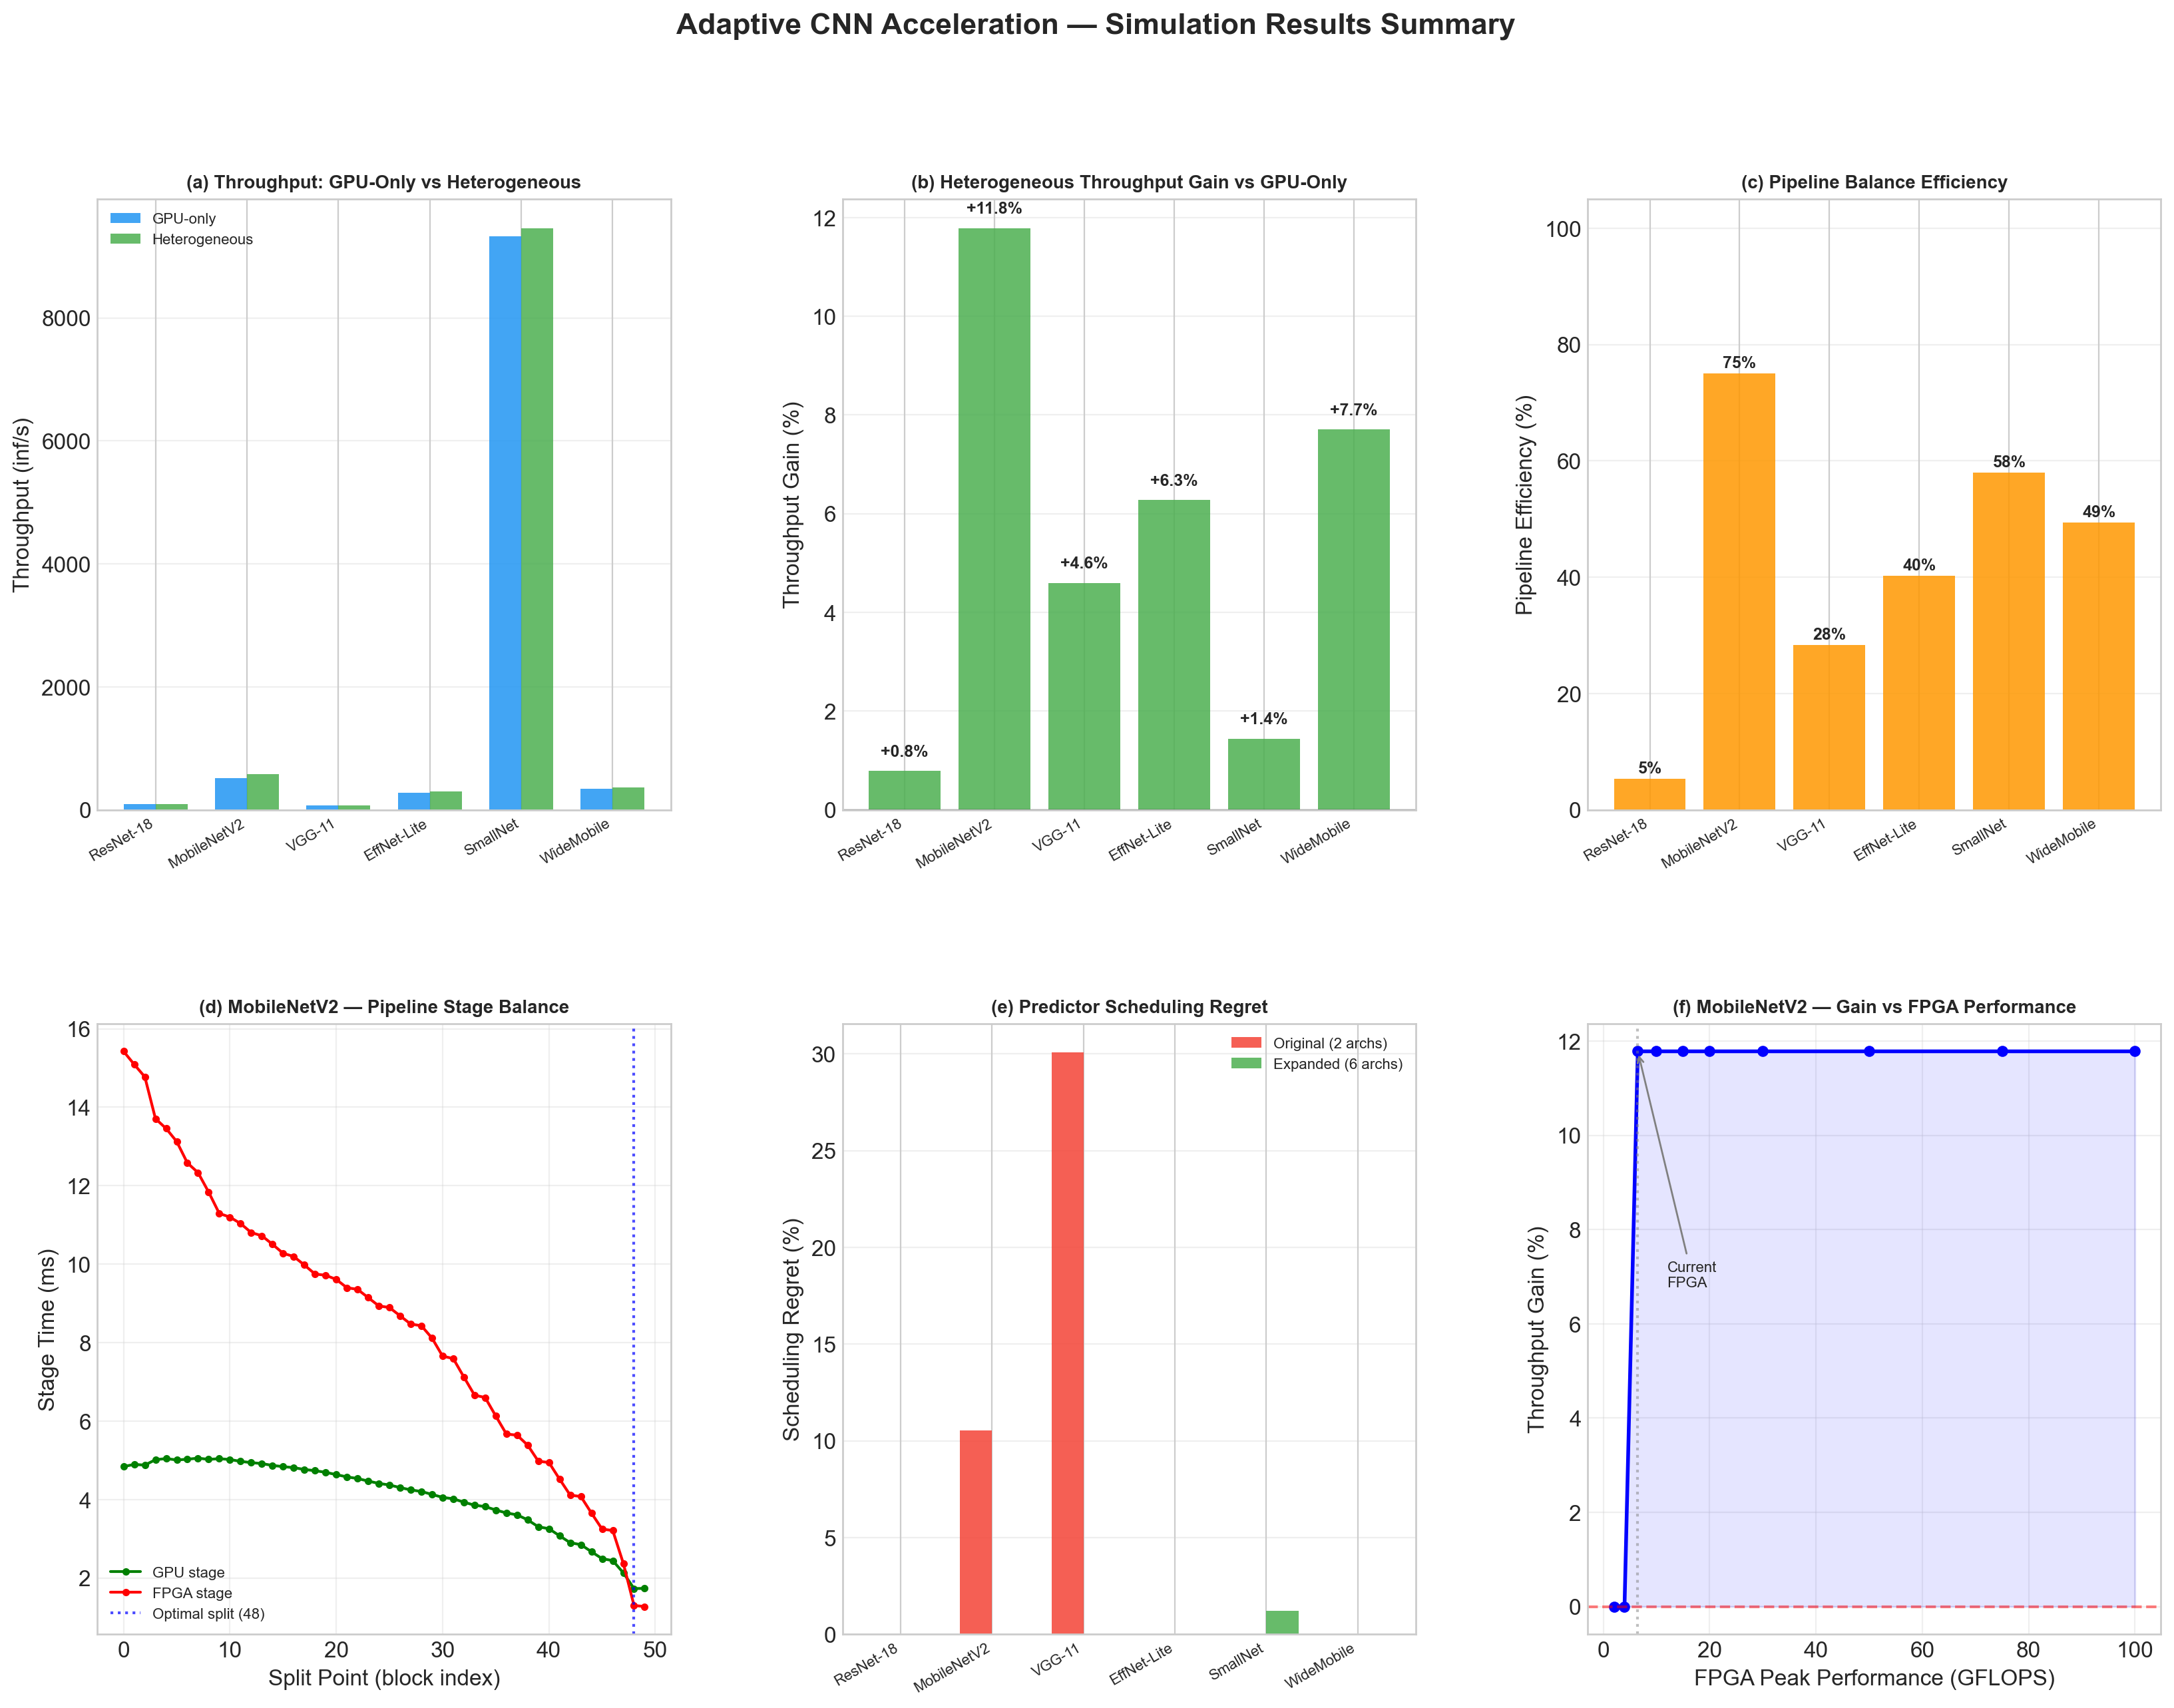
\includegraphics[width=\textwidth]{final_results_summary.png}
\caption{Trial 1 summary: (a) throughput comparison, (b) heterogeneous gain per architecture, (c) pipeline efficiency, (d) MobileNetV2 stage balance, (e) predictor regret improvement, (f) gain vs FPGA scaling.}\label{fig:t1_summary}
\end{figure}

A calibration predictor trained on 735 samples achieved 0.20\% average in-model scheduling regret (Table~\ref{tab:predictor}). Expanding training from 2 to 6 architectures reduced regret from 6.77\% to 0.20\% (Fig.~\ref{fig:t1_predictor} in Appendix). Multi-split partitioning (2--3 splits) provided no improvement over single-split for any architecture (Fig.~\ref{fig:t1_multisplit} in Appendix).

\begin{table}
\caption{Calibration predictor accuracy (in-model protocol; cf. Section~\ref{sec:b5}).}\label{tab:predictor}
\centering
\begin{tabular}{lccc}
\toprule
\textbf{Architecture} & \textbf{Oracle} & \textbf{Predicted} & \textbf{Regret} \\
\midrule
ResNet-18 & 17 & 17 & 0.00\% \\
MobileNetV2 & 48 & 48 & 0.00\% \\
VGG-11 & 14 & 14 & 0.00\% \\
EfficientNet-Lite & 21 & 21 & 0.00\% \\
SmallCustomNet & 6 & 7 & 1.21\% \\
WideMobileNet & 24 & 24 & 0.00\% \\
\midrule
\textbf{Average} & & & \textbf{0.20\%} \\
\bottomrule
\end{tabular}
\end{table}

\subsection{Trial 2: Functional Emulation}\label{sec:trial2}

The FPGA emulator models a sequential streaming pipeline with 220 DSP slices; the GPU emulator models parallel batch processing across 128 CUDA cores.

\subsubsection{Memory-Bound Reality.} All layers on both architectures are memory-bound on the FPGA (compute/memory ratio: 0.10 ResNet, 0.01 MobileNet). The emulated FPGA/GPU ratio is 2.27$\times$ (ResNet) and 1.61$\times$ (MobileNet); after fusion+INT8, 1.00$\times$ and 1.49$\times$ (Fig.~\ref{fig:t2_perlayer}).

\begin{figure}[t]
\centering
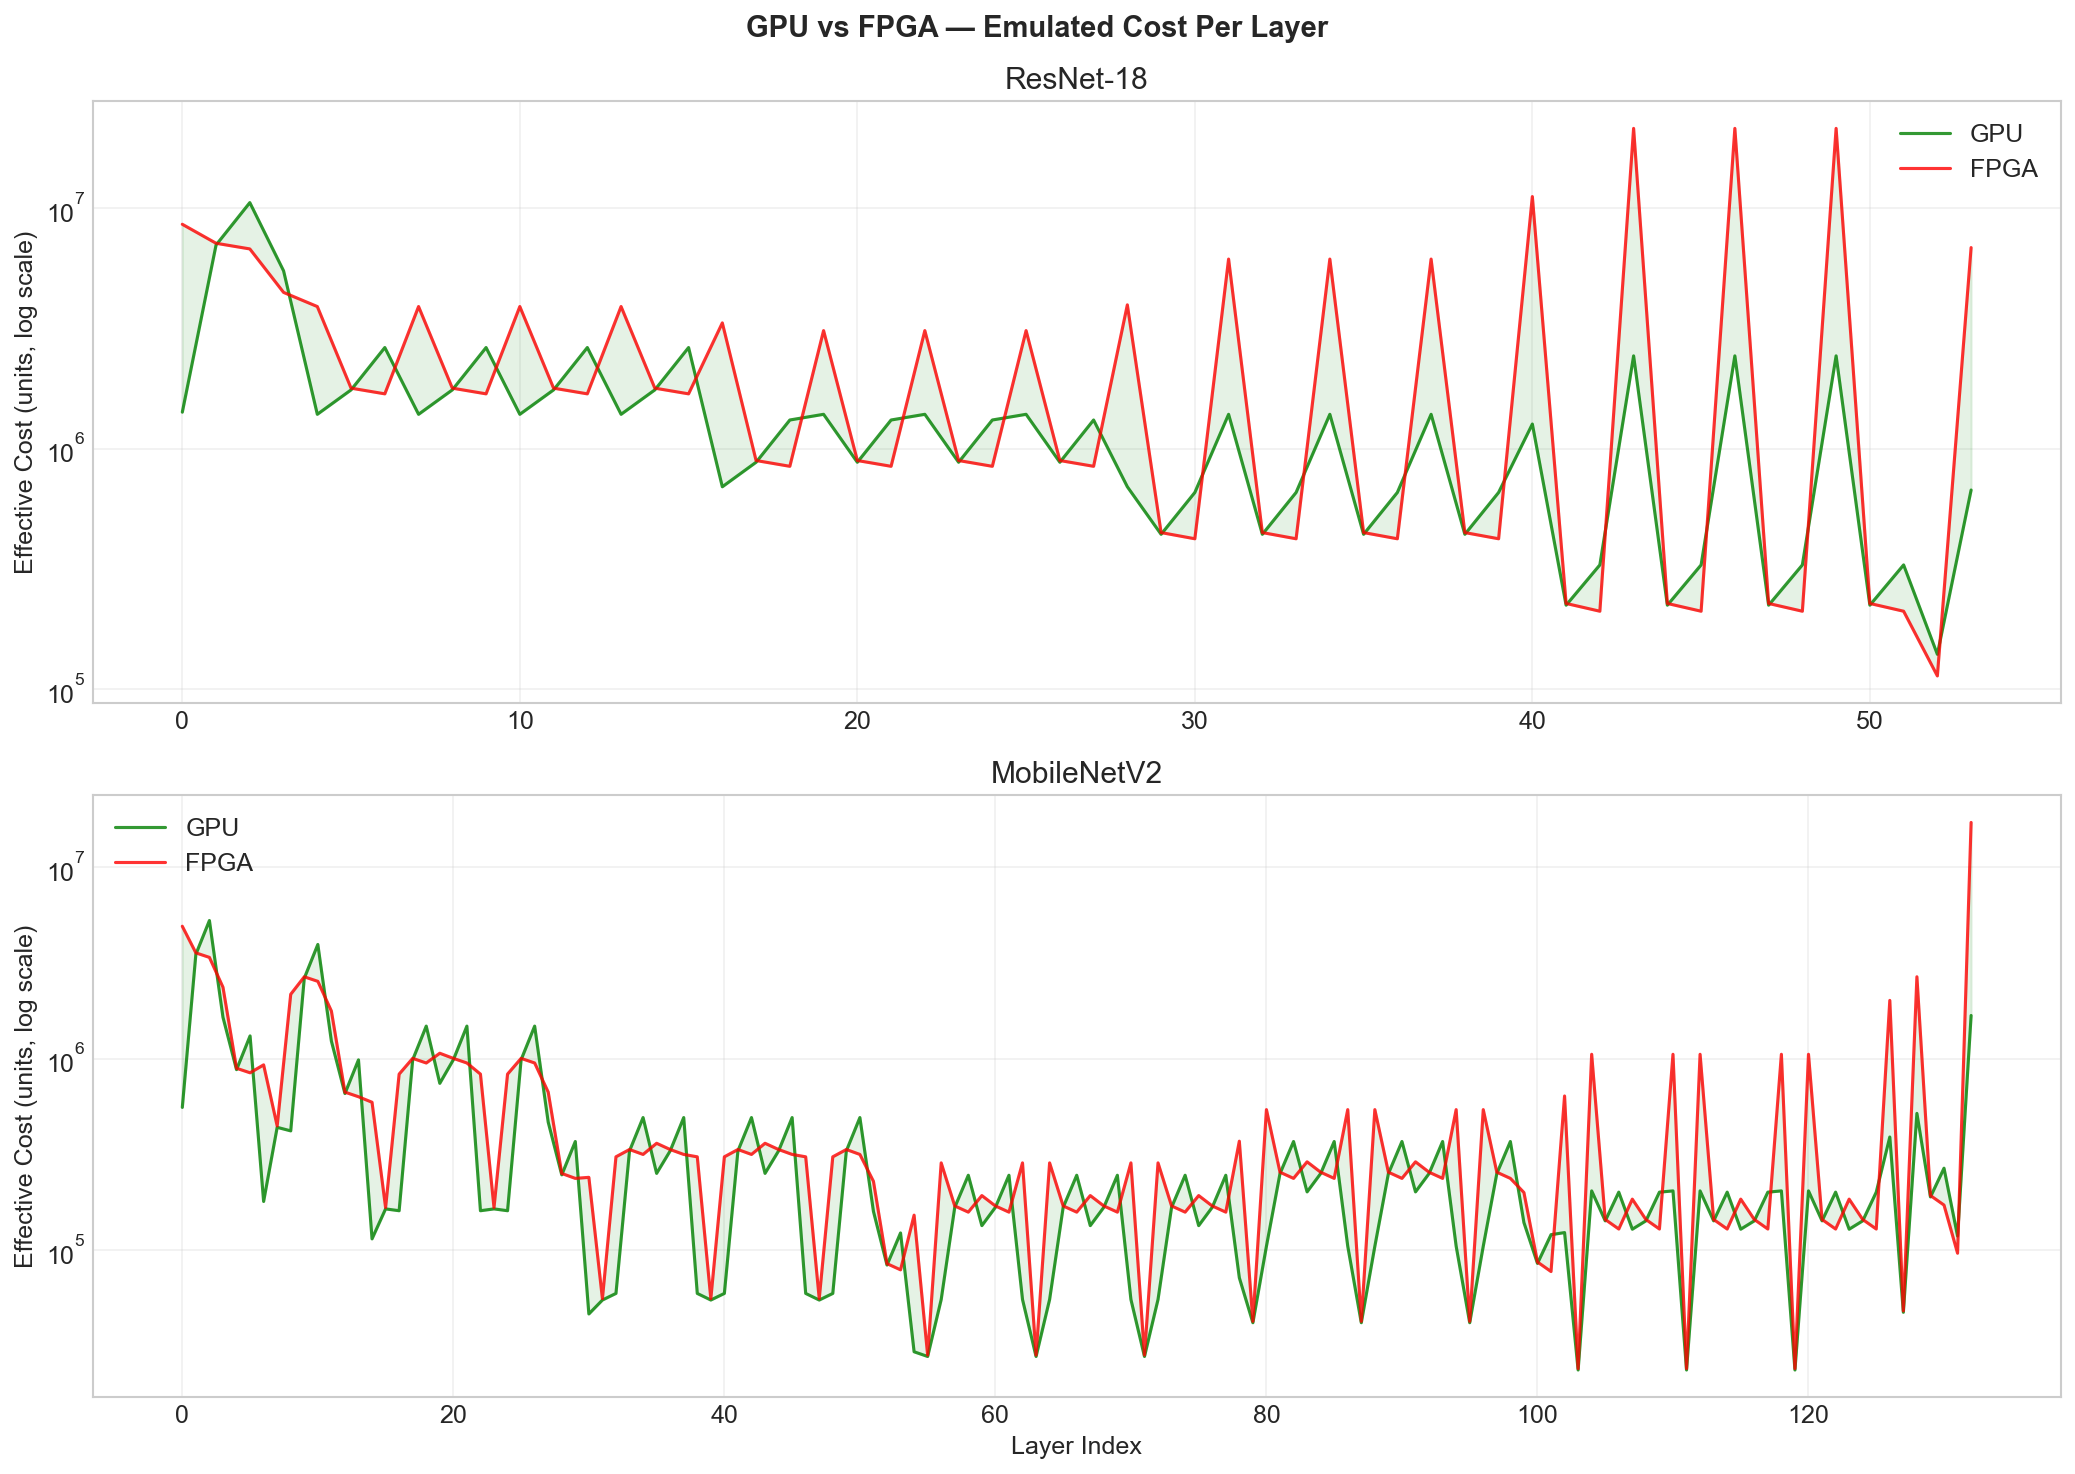
\includegraphics[width=\textwidth]{gpu_vs_fpga_per_layer.png}
\caption{Emulated per-layer cost: GPU vs FPGA on log scale for ResNet-18 (top) and MobileNetV2 (bottom).}\label{fig:t2_perlayer}
\end{figure}

\subsubsection{Fusion Savings.} Emulated fusion saves 47\% (GPU) and 77\% with INT8 (FPGA) for ResNet-18, and 64\% (GPU) and 66\% (FPGA) for MobileNetV2 (Fig.~\ref{fig:t2_fusion} in Appendix). These far exceed the analytical model's 20\% because eliminating intermediate tensor I/O has outsized impact in the memory-bound regime.

\subsubsection{Pipeline Results.} The optimizer finds +75\% gain for ResNet-18 (split at block 13, 96.6\% efficiency) and +10.1\% for MobileNetV2 (block 48, 96.8\%). Streaming simulation of 100 inferences confirms +73.3\% and +9.1\% sustained gain with both devices above 95\% utilization (Figs.~\ref{fig:t2_streaming} and~\ref{fig:t2_pipeline} in Appendix).

\begin{figure}[t]
\centering
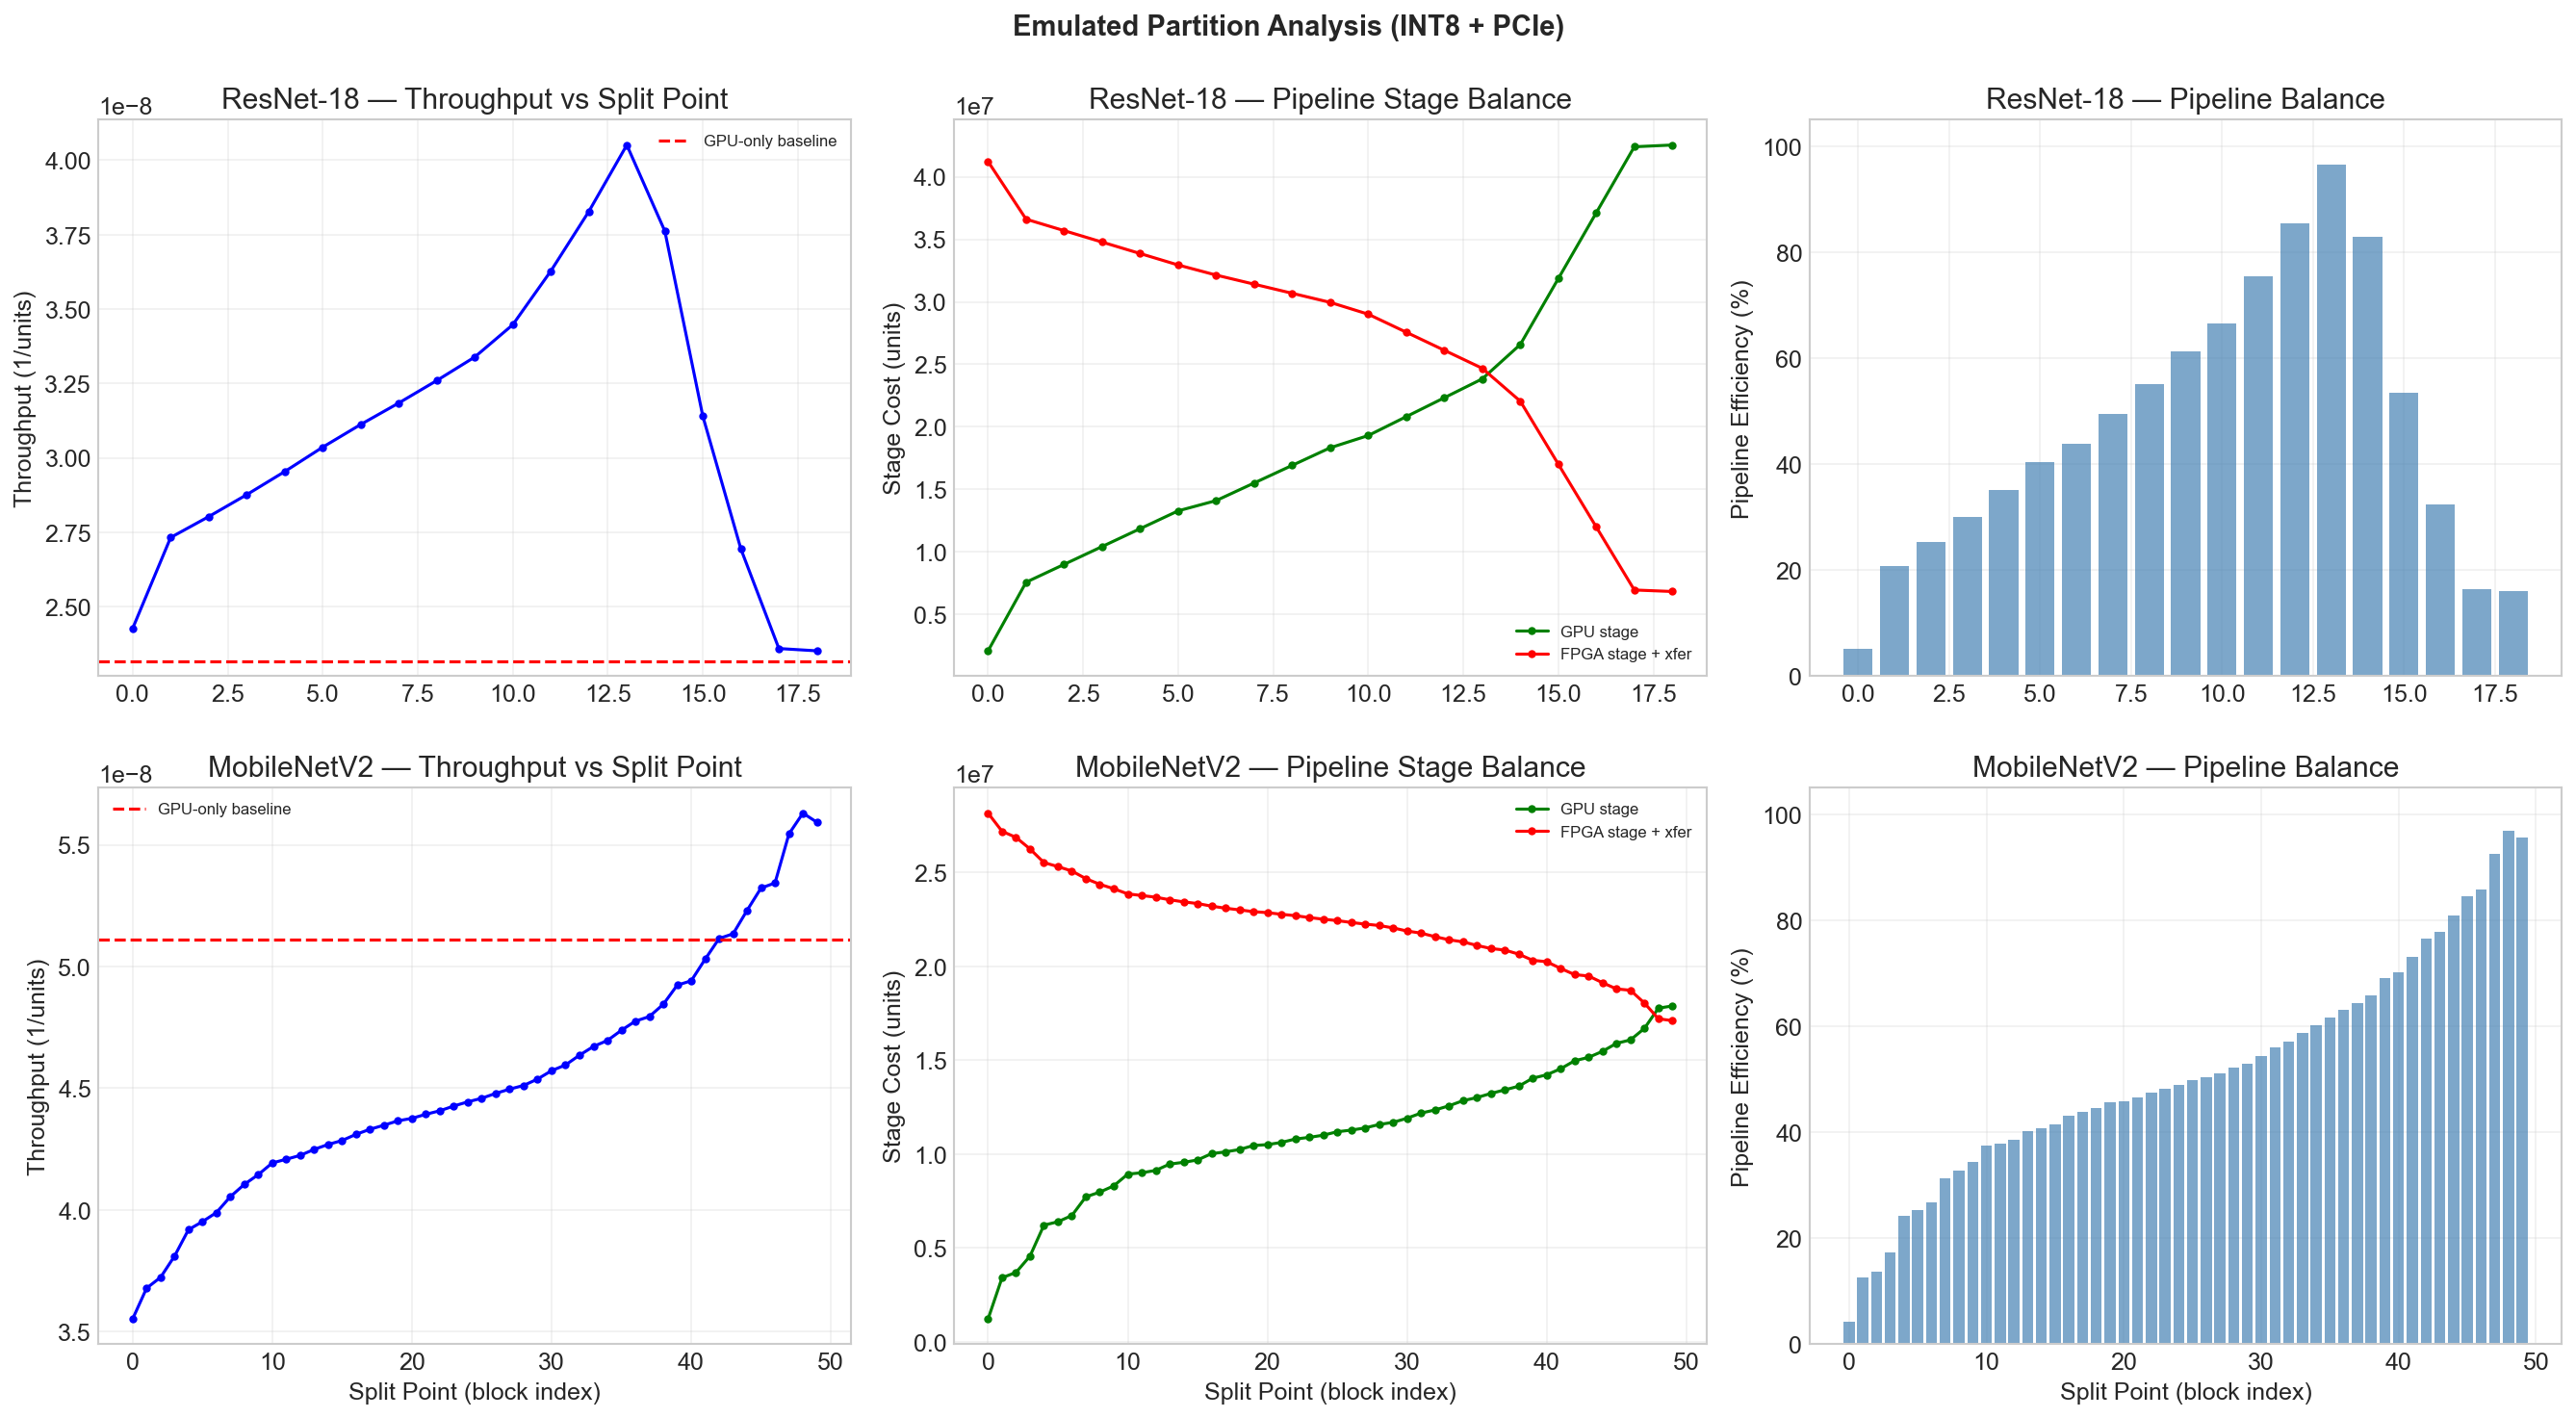
\includegraphics[width=\textwidth]{emulated_partition_analysis.png}
\caption{Emulated partition analysis: throughput, stage balance, and efficiency across split points.}\label{fig:t2_partition}
\end{figure}

\subsection{Analytical vs Emulated Comparison}\label{sec:comparison}

Table~\ref{tab:threelevels} and Fig.~\ref{fig:t2_comparison} compare key metrics between the two modeling levels.

\begin{table}
\caption{Comparison across the analytical and emulated modeling levels.}\label{tab:threelevels}
\centering
\begin{tabular}{lcccc}
\toprule
\textbf{Metric} & \multicolumn{2}{c}{\textbf{ResNet-18}} & \multicolumn{2}{c}{\textbf{MobileNetV2}} \\
 & Analyt. & Emul. & Analyt. & Emul. \\
\midrule
FPGA/GPU ratio & 36.9$\times$ & 1.00$\times$ & 9.4$\times$ & 1.49$\times$ \\
Throughput gain & +0.8\% & +73.3\% & +11.8\% & +9.1\% \\
Pipeline eff. & 5\% & 96.6\% & 75\% & 96.8\% \\
Fusion savings & 20\% & 47\% & 20\% & 64\% \\
Optimal split & 17 & 13 & 48 & 48 \\
\bottomrule
\end{tabular}
\end{table}

\begin{figure}[t]
\centering
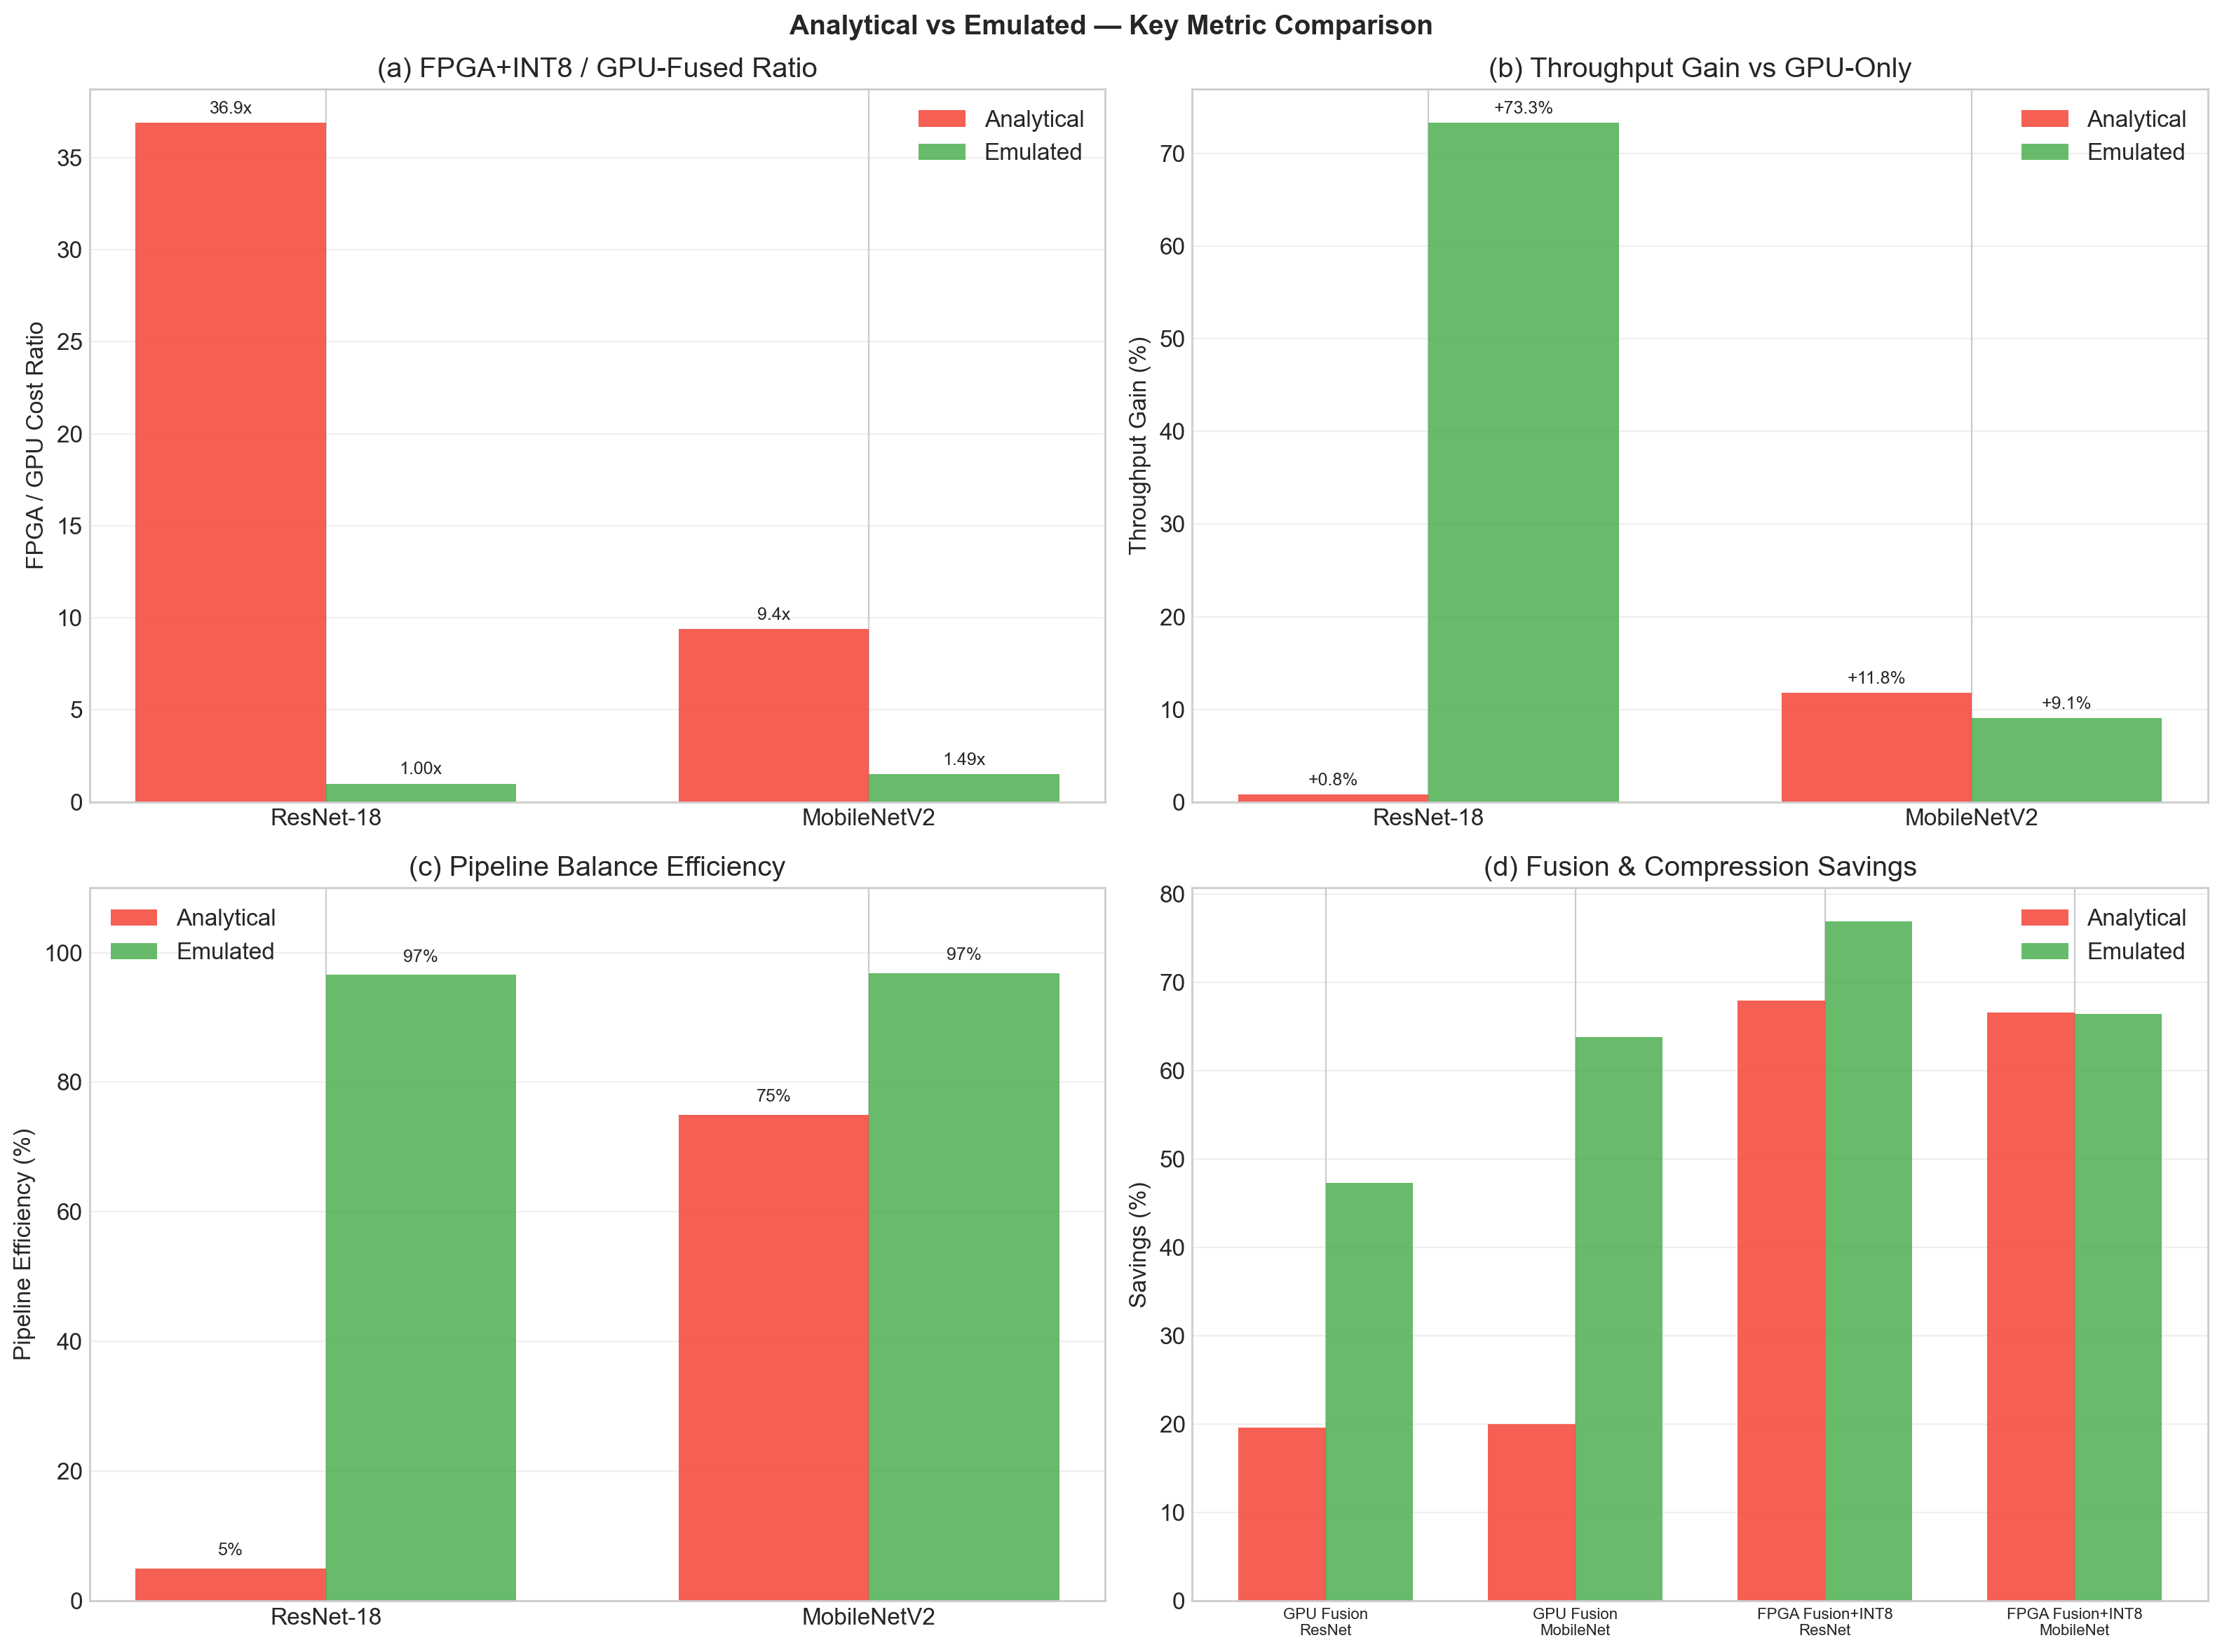
\includegraphics[width=\textwidth]{analytical_vs_emulated_comparison.png}
\caption{Analytical vs emulated: (a) FPGA/GPU ratio, (b) throughput gain, (c) pipeline efficiency, (d) fusion savings.}\label{fig:t2_comparison}
\end{figure}

\subsection{Calibrated Results and Break-Even}\label{sec:calibrated}

Emulated costs were calibrated against published benchmarks---edge-GPU inference times from TensorRT~\cite{tensorrt} and edge-device studies such as DeepEdgeBench~\cite{deepedgebench2021}, and embedded-FPGA CNN latencies of the Zynq class~\cite{qiu2016} (ResNet-18: 26~ms Jetson Nano, 202~ms Zynq~7020; MobileNetV2: 10~ms, 43~ms)---using Eq.~\eqref{eq:calibration}. Local RTX 4070 measurements provided cross-validation (<9\% GPU error). FPGA factors differed 3.2$\times$ between architectures.

Break-even requires 1.5$\times$ for ResNet-18 (6.7 GMAC/s) and 3.0$\times$ for MobileNetV2 (6.3 GMAC/s). UltraScale+ at 5--8$\times$ yields substantial gains (Table~\ref{tab:projection}, Fig.~\ref{fig:t2_sensitivity}).

\begin{table}
\caption{Projected gains on UltraScale+ (emulated model).}\label{tab:projection}
\centering
\begin{tabular}{lcccc}
\toprule
\textbf{Arch.} & \textbf{5$\times$ Gain} & \textbf{5$\times$ Eff.} & \textbf{8$\times$ Gain} & \textbf{8$\times$ Eff.} \\
\midrule
ResNet-18 & +35.6\% & 90.5\% & +65.3\% & 91.2\% \\
MobileNetV2 & +66.5\% & 99.4\% & +139.9\% & 97.7\% \\
\bottomrule
\end{tabular}
\end{table}

\begin{figure}[t]
\centering
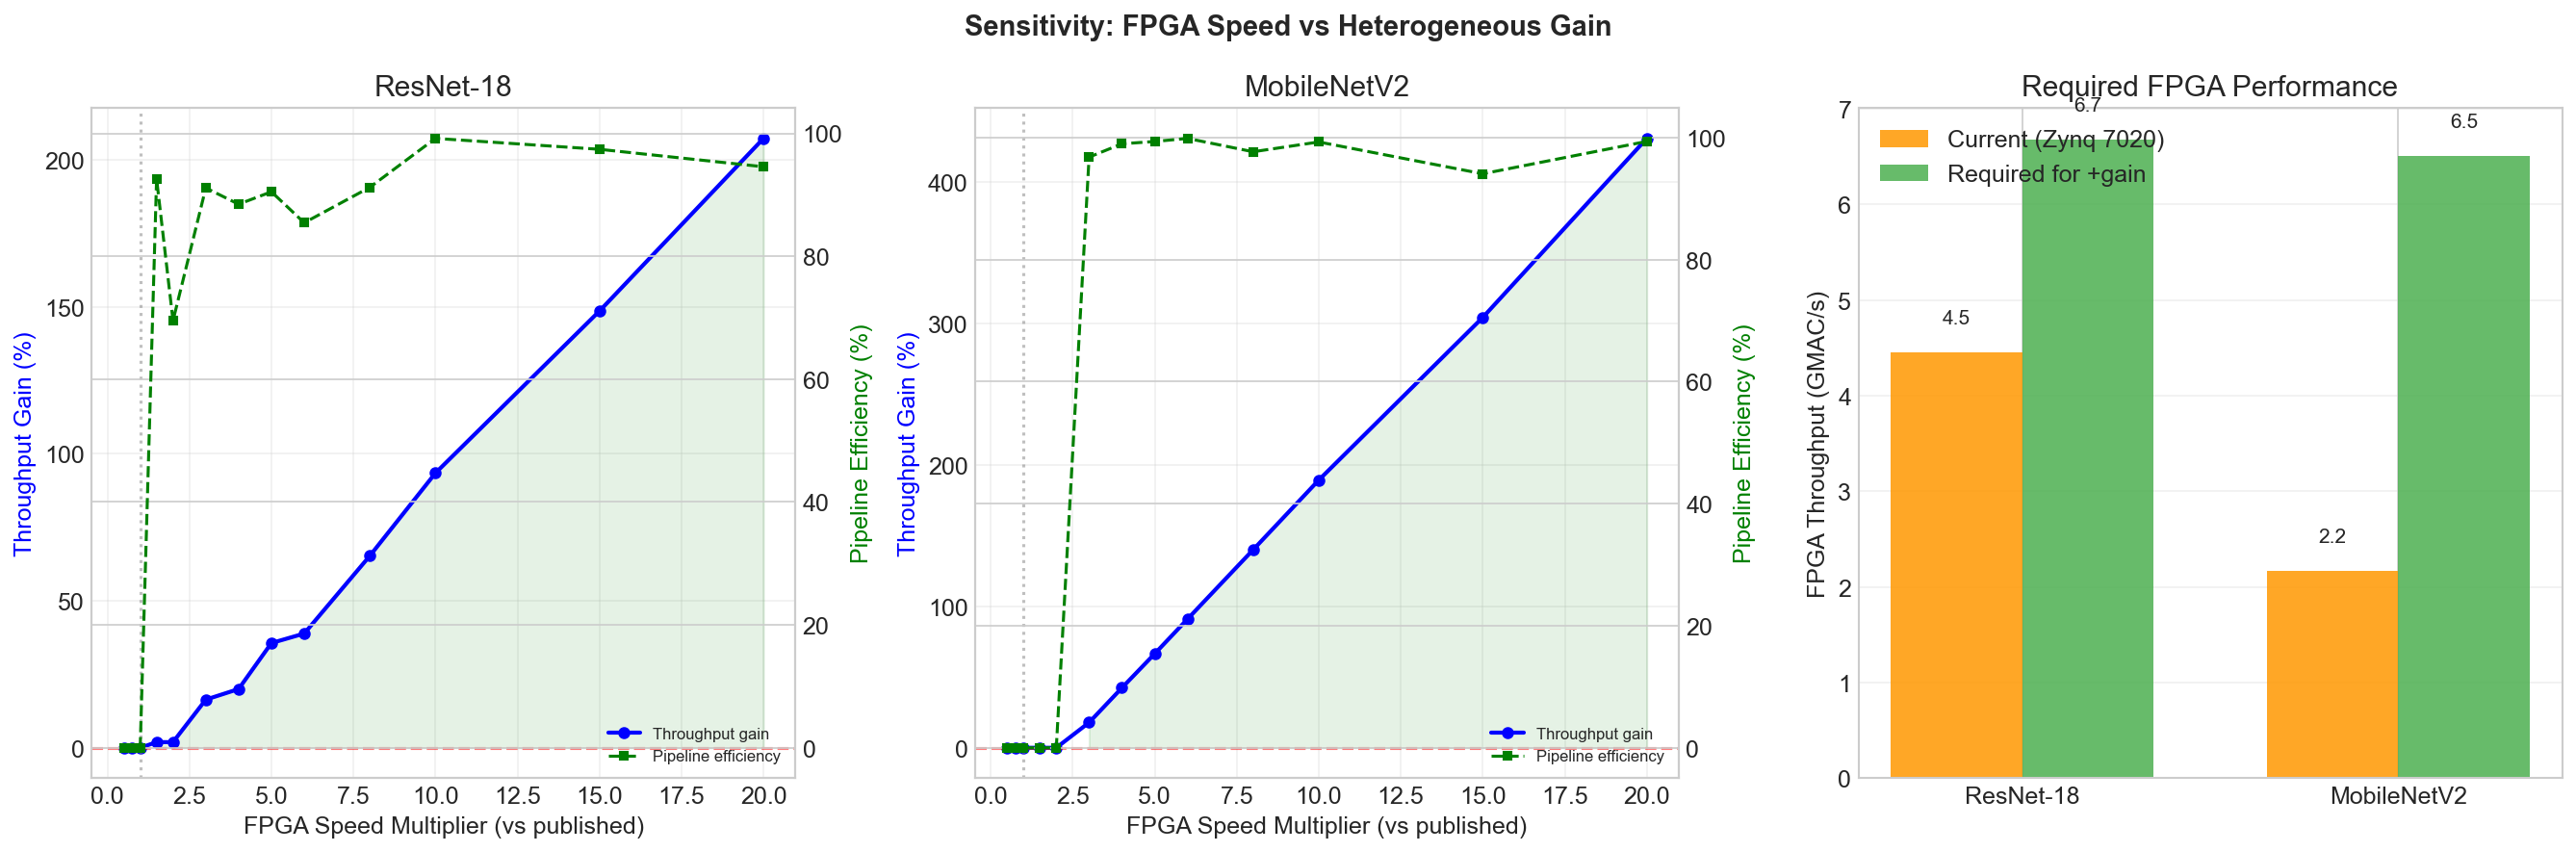
\includegraphics[width=\textwidth]{sensitivity_fpga_speed.png}
\caption{FPGA speed sensitivity: throughput gain vs speed multiplier and required GMAC/s for break-even.}\label{fig:t2_sensitivity}
\end{figure}

Additional calibrated projections and the complete Trial~2 summary are provided in Figs.~\ref{fig:t2_calibrated} and~\ref{fig:t2_final} in the Appendix.

\section{Trial 3: Hardware-Grounded Evaluation}\label{sec:grounded}

Trials~1--2 rest on the hand-set efficiency factors of Table~\ref{tab:efficiency} and on an extrapolated break-even projection. Trial~3 replaces the hand-set factors with values obtained directly from synthesis and measurement, then tests whether the heterogeneous benefit survives, calibrates the two grounded models to a common time base, and quantifies the pipeline realism, uncertainty, and accuracy cost that determine practical attainability.

\subsection{FPGA Cost Grounding via HLS Synthesis}\label{sec:hls}

We implemented INT8 streaming kernels for the seven operator types (standard/depthwise/pointwise convolution, batch normalization, ReLU, pooling, fully connected) in C++ and synthesized them with AMD Vitis HLS~2026.1~\cite{vitishls} targeting the Zynq-7020 part (\texttt{xc7z020-clg400-1}) at 100~MHz, in the spirit of HLS accelerator generators such as FINN~\cite{finn2017} and hls4ml~\cite{hls4ml2018} but used here to \emph{cost} operators rather than to build a full accelerator. C-synthesis runs entirely on CPU and requires no board. For each operator we take a device-\emph{fitting} design point and define a compute efficiency as achieved MACs-per-cycle normalized by the 220-DSP peak (the same scale as the hand-set $\eta_{\text{FPGA}}$); a memory bandwidth in bytes/cycle is extracted from the memory-bound kernels (ReLU/BN/pool). The FPGA cost is then the roofline $\max(\text{compute}, \text{memory})$.

Two findings emerge. First, the memory-bound operators (depthwise convolution, BN, ReLU, pool) do not benefit from added parallelism: unrolling them merely consumes DSPs without raising throughput, so their efficient realization is a narrow streaming datapath. Second, the convolution datapath is decisive. An initial \emph{naive} convolution kernel exhibited a sharp DSP cliff---a single unroll knob forced HLS to fully unroll the entire reduction, so it fit the 7020 only at a near-serial 6-DSP point and exploded past 322 DSPs at any higher setting---making convolution appear far more expensive on the FPGA than it need be. We therefore designed an \emph{output-stationary, DSP-tiled} convolution (separate output- and input-channel tiles $T_M,T_N$, int8$\times$int8 MACs, a zero-padded on-chip buffer). Its resource use scales gracefully ($40\to72\to166$ DSPs as $T_M\!\cdot\!T_N$ grows), and the best point that fits the device ($T_M{=}16,T_N{=}8$: 72 DSPs) reaches $\sim$63 MACs/cycle---a convolution efficiency of $\approx0.29$, roughly $21\times$ the naive kernel and comparable to the GPU, with \emph{BRAM} (the on-chip cache), not DSP, now the binding constraint (Fig.~\ref{fig:grounded}, right).

We validated this kernel end-to-end (item extending beyond C-synthesis): C-simulation against a reference convolution matches on all $200{,}704$ outputs, and Vivado out-of-context synthesis and place-and-route on the \texttt{xc7z020} yields 73 DSPs, 11{,}011 LUTs, 258/280 BRAM (92\%), meeting timing at 100~MHz (post-route critical path 9.87~ns). The implemented resource figures confirm the C-synthesis estimates and that the design physically fits the target part.

\subsection{GPU Cost Grounding}\label{sec:gpu}

The GPU per-op efficiency was measured directly on an NVIDIA RTX~4070 Laptop GPU, timing each operator type at batch~1 on the same representative shapes with CUDA events (warmup plus median over 200 runs) and normalizing achieved MAC throughput to the best operator (dense convolution). The measured pattern is far more skewed than the hand-set values: convolution reaches unit efficiency, while pointwise (0.12), depthwise (0.06), pooling (0.05), and the elementwise/FC operators ($\sim$0.007) are much lower, since at batch~1 the small and memory-bound operators are kernel-launch bound.

\subsection{Grounded Partition Results}\label{sec:grounded_results}

Substituting the synthesized FPGA efficiencies (GPU model held at the hand-set values, to isolate the FPGA grounding) and re-running the optimizer gives large gains for \emph{both} architecture classes once the tiled convolution is used (Table~\ref{tab:grounded}, Fig.~\ref{fig:grounded}). These are \emph{unit-space} (relative) gains; the absolute-time picture, which is stricter, follows from the calibration in Section~\ref{sec:b6}. For MobileNetV2 the grounded FPGA cost is close to the GPU cost (FPGA/GPU $\approx 0.8\times$), so the pipeline balances and throughput approximately doubles ($+102\%$). For ResNet-18 the tiled convolution makes the FPGA cost \emph{lower} than the GPU cost (FPGA/GPU $\approx 0.8\times$)---its many BN/ReLU/pool layers are cheap on the FPGA while its convolutions are now competitive---so the pipeline likewise balances and throughput more than doubles ($+155\%$). For reference, with the earlier naive convolution ResNet-18 offloaded only a small tail ($+9\%$, FPGA/GPU $\approx 14\times$); the $17\times$ swing between the two kernels is the clearest evidence that the convolution datapath, not the device, governed the earlier pessimistic verdict.

\begin{table}
\caption{Throughput gain vs GPU-only and FPGA/GPU cost ratio across the three modeling levels. Trial~3 uses HLS-synthesized FPGA costs (GPU hand-set, to isolate the FPGA grounding).}\label{tab:grounded}
\centering
\begin{tabular}{lcccc}
\toprule
\textbf{Level} & \multicolumn{2}{c}{\textbf{ResNet-18}} & \multicolumn{2}{c}{\textbf{MobileNetV2}} \\
 & Gain & FPGA/GPU & Gain & FPGA/GPU \\
\midrule
Analytical (Trial 1) & +0.8\% & 36.9$\times$ & +11.8\% & 9.4$\times$ \\
Emulated (Trial 2) & +75.0\% & 1.0$\times$ & +10.1\% & 1.5$\times$ \\
Grounded (Trial 3) & +155.2\% & 0.8$\times$ & +102.2\% & 0.8$\times$ \\
\bottomrule
\end{tabular}
\end{table}

\begin{figure}[t]
\centering
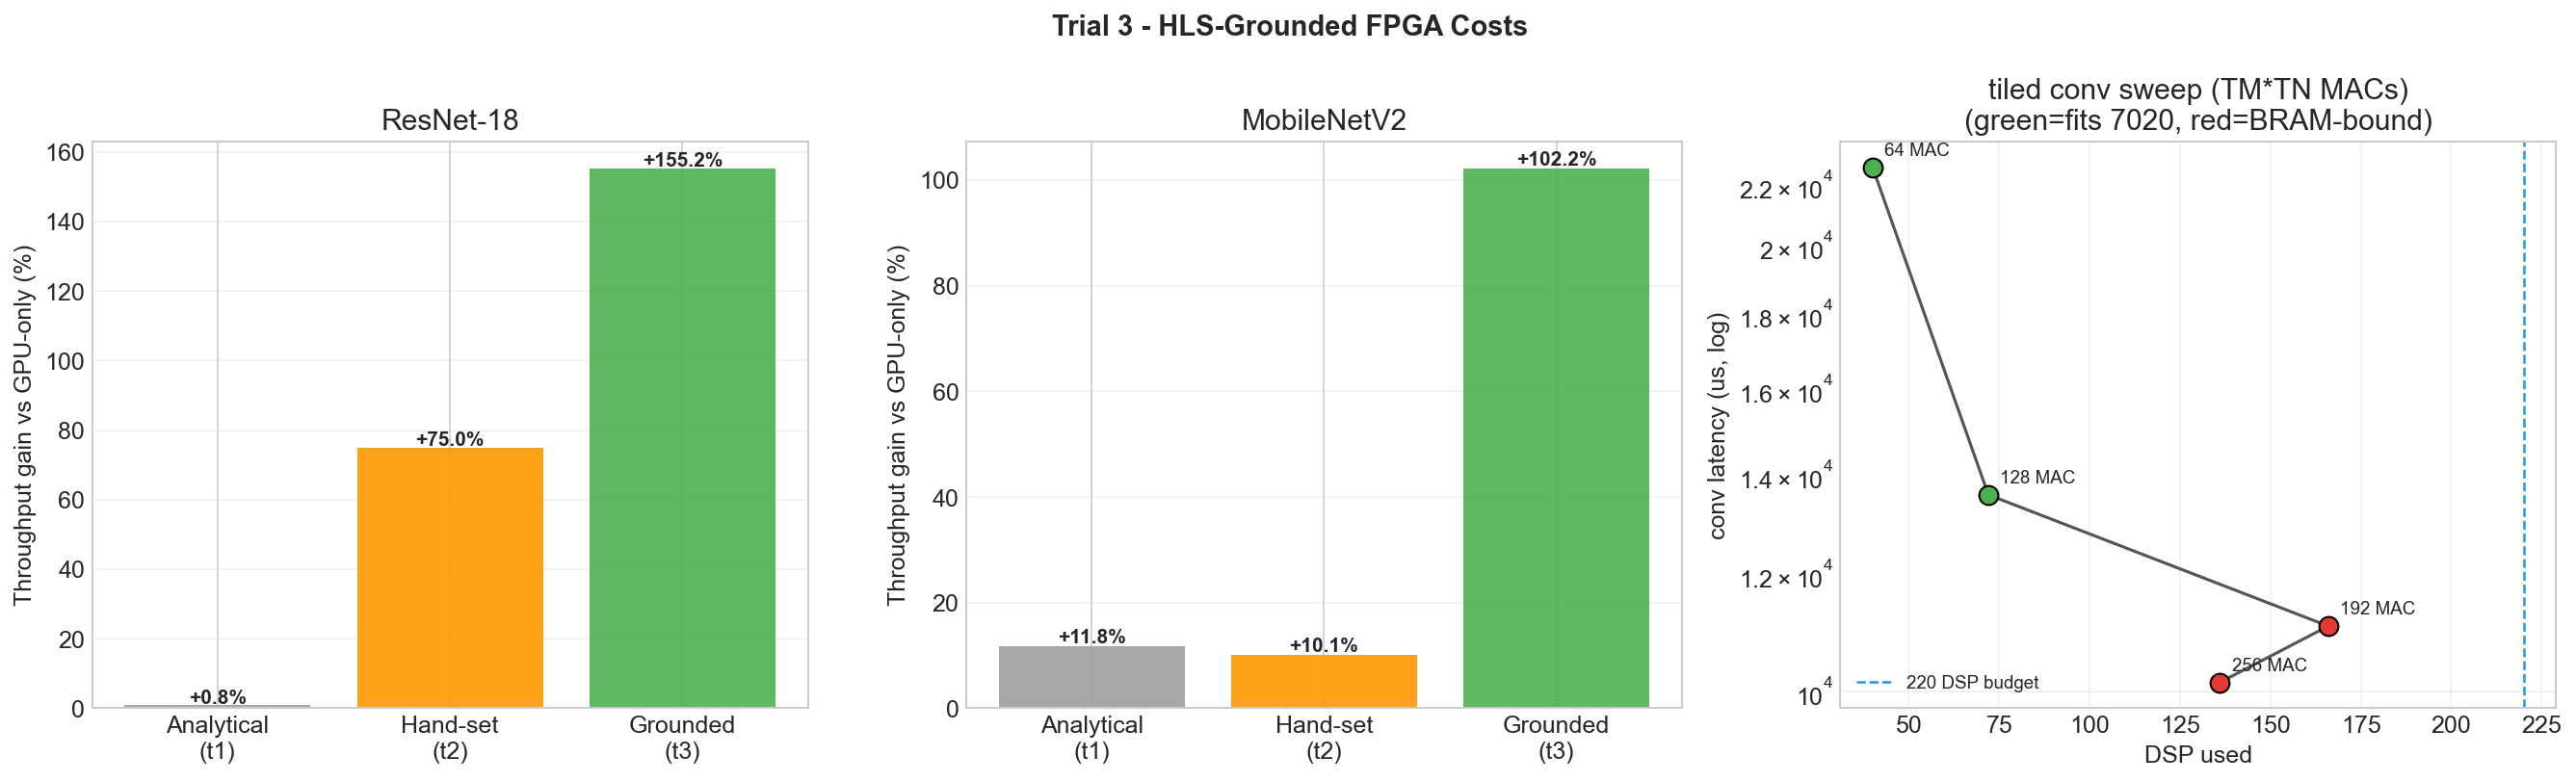
\includegraphics[width=\textwidth]{grounded_three_way_comparison.png}
\caption{Hardware-grounded results: throughput gain across the three modeling levels for ResNet-18 (left) and MobileNetV2 (center), and the tiled-convolution $T_M\!\cdot\!T_N$ sweep (right; green fits the 7020, red is BRAM-bound). The tiled kernel scales gracefully with no DSP cliff.}\label{fig:grounded}
\end{figure}

\subsection{Cross-Device Calibration}\label{sec:b6}

The grounded gains reported so far are in \emph{unit space} (relative per-op cost structure): they assume a GPU-unit and an FPGA-unit take equal wall-clock time, which they do not. Calibrating each device's units to \emph{milliseconds} against published anchors (Eq.~\eqref{eq:calibration}; GPU 26/60~ms, FPGA 202/43~ms for ResNet-18/MobileNetV2) tells a stricter, absolute-time story and also resolves the fact that grounding both devices in raw unit space inflates the apparent MobileNetV2 gain to over $1400\%$. Calibrated to the \emph{current} Zynq~7020, only MobileNetV2 is net-positive ($+52\%$); ResNet-18 is $\mathbf{-79\%}$---its heavier convolution workload, offloaded to an absolutely slow device, costs wall-clock even though the relative structure favours the split. This directly reaffirms the break-even analysis of Section~\ref{sec:calibrated}: conv-heavy networks need a faster FPGA (UltraScale+ class) to convert their favourable relative structure into an absolute win. A leave-one-out check further shows FPGA milliseconds-per-unit does \emph{not} transfer across architectures (54.8\% and 121.4\% held-out error), whereas the GPU factor is stable---corroborating that FPGA cost is workload-specific and GPU cost is not.

\subsection{Latency Predictor Revisited}\label{sec:b5}

We re-evaluate the scheduling predictor of Section~\ref{sec:predictor} under a protocol that removes the circularity of the in-model result. Rather than training and testing on the analytical formula plus noise, we predict the \emph{synthesized} per-block FPGA cost from block features and evaluate by \emph{leave-one-architecture-out} cross-validation across four networks. Scheduling regret is 0\% for the conv-heavy ResNet-18 and VGG-11 but 21.6\% and 26.5\% for the depthwise-heavy MobileNetV2 and EfficientNet-Lite (prediction error up to 121\% MAPE). This 0--26\% range is the honest generalization figure; the 0.20\% of Table~\ref{tab:predictor} reflects a predictor recovering the cost function it was trained on, not transfer to unseen workloads.

\subsection{Uncertainty Analysis}\label{sec:d8}

The synthesized constants are point estimates from single design points. We place lognormal uncertainty on the FPGA per-op efficiencies ($\sigma{=}0.4$), FPGA memory bandwidth ($\sigma{=}0.3$), and transfer bandwidth ($\sigma{=}0.2$), and resample the optimal-split gain 3000 times (Fig.~\ref{fig:montecarlo}). The gain is $+8.7\%$ for ResNet-18 (90\% CI $[+1.9\%, +16.4\%]$) and $+101\%$ for MobileNetV2 ($[+64\%, +152\%]$), with $P(\text{gain}>0)=100\%$ for both: the sign of the benefit is robust to constant uncertainty, though the magnitude is not sharp.

\begin{figure}[t]
\centering
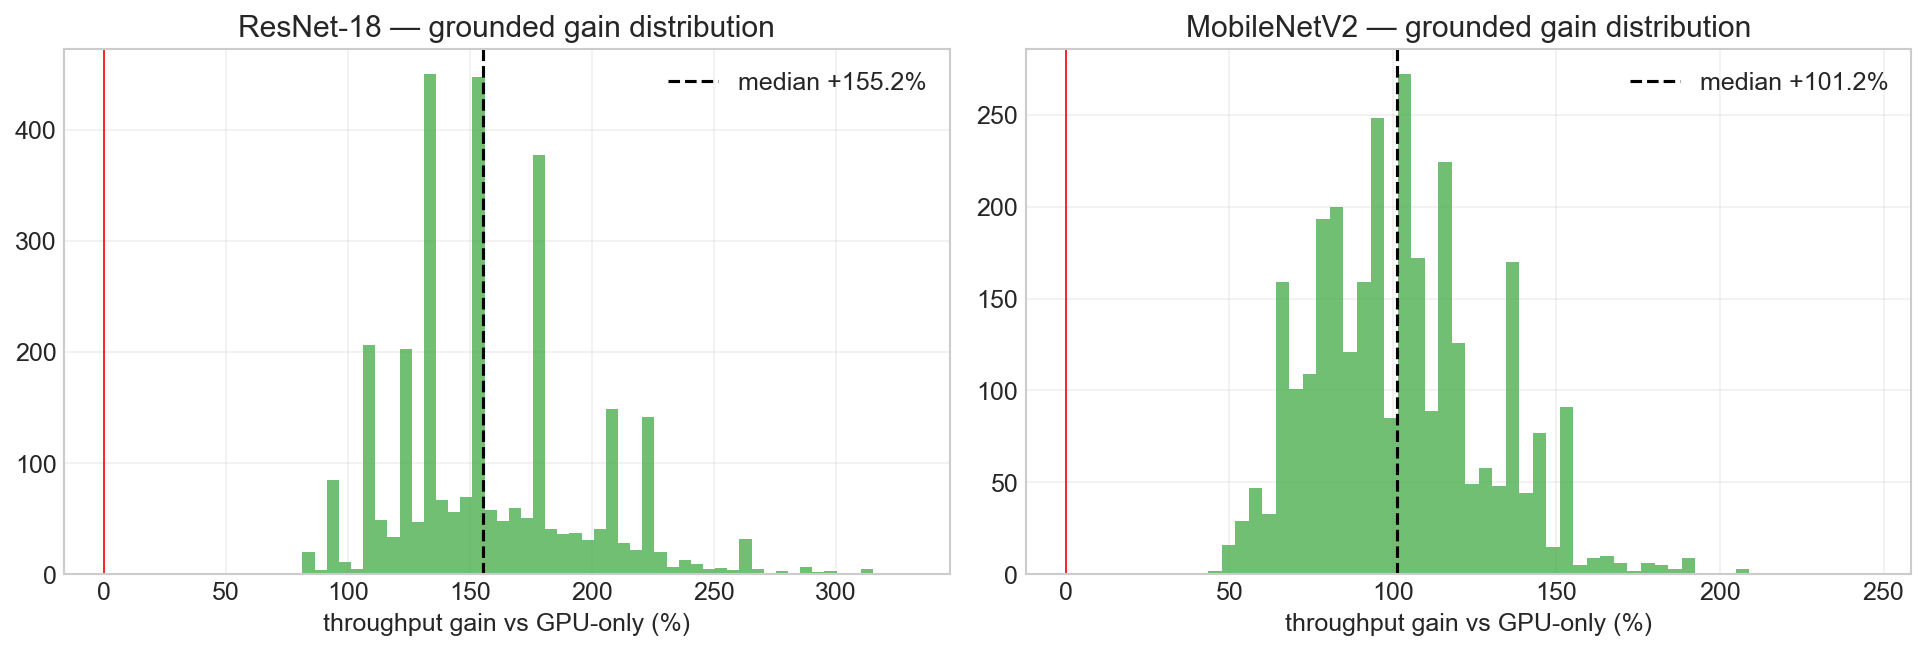
\includegraphics[width=\textwidth]{grounded_montecarlo.png}
\caption{Monte-Carlo distribution of the grounded throughput gain (3000 samples) for ResNet-18 (left) and MobileNetV2 (right). Dashed line: median; red line: zero gain.}\label{fig:montecarlo}
\end{figure}

\subsection{Pipeline Realism}\label{sec:e10}

Equation~\eqref{eq:throughput} assumes perfect overlap, infinite buffering, and an infinite stream. We relax all three with a discrete-event simulation of a finite stream through a two-stage line (GPU; FPGA+transfer) with a finite inter-stage buffer, blocking-after-service, and per-item service-time variability (Fig.~\ref{fig:pipesim}). With an infinite buffer, deterministic times, and $N\to\infty$ it reproduces the idealized ceiling; finite effects only reduce it. At a realistic 64-frame stream with buffer~2 and coefficient of variation~0.2, both unit-space gains survive the tempering: ResNet-18 falls from $+155\%$ to $+132\%$ and MobileNetV2 from $+102\%$ to $+81\%$ (relative structure; the absolute-time verdict is in Section~\ref{sec:b6}). (As a contrast, with the earlier naive convolution ResNet-18's marginal $+9\%$ instead evaporated to $\approx 0\%$ here---a concrete illustration of how kernel quality propagates all the way to the sustained-throughput verdict.) Both benefits are robust to realistic pipeline effects.

\begin{figure}[t]
\centering
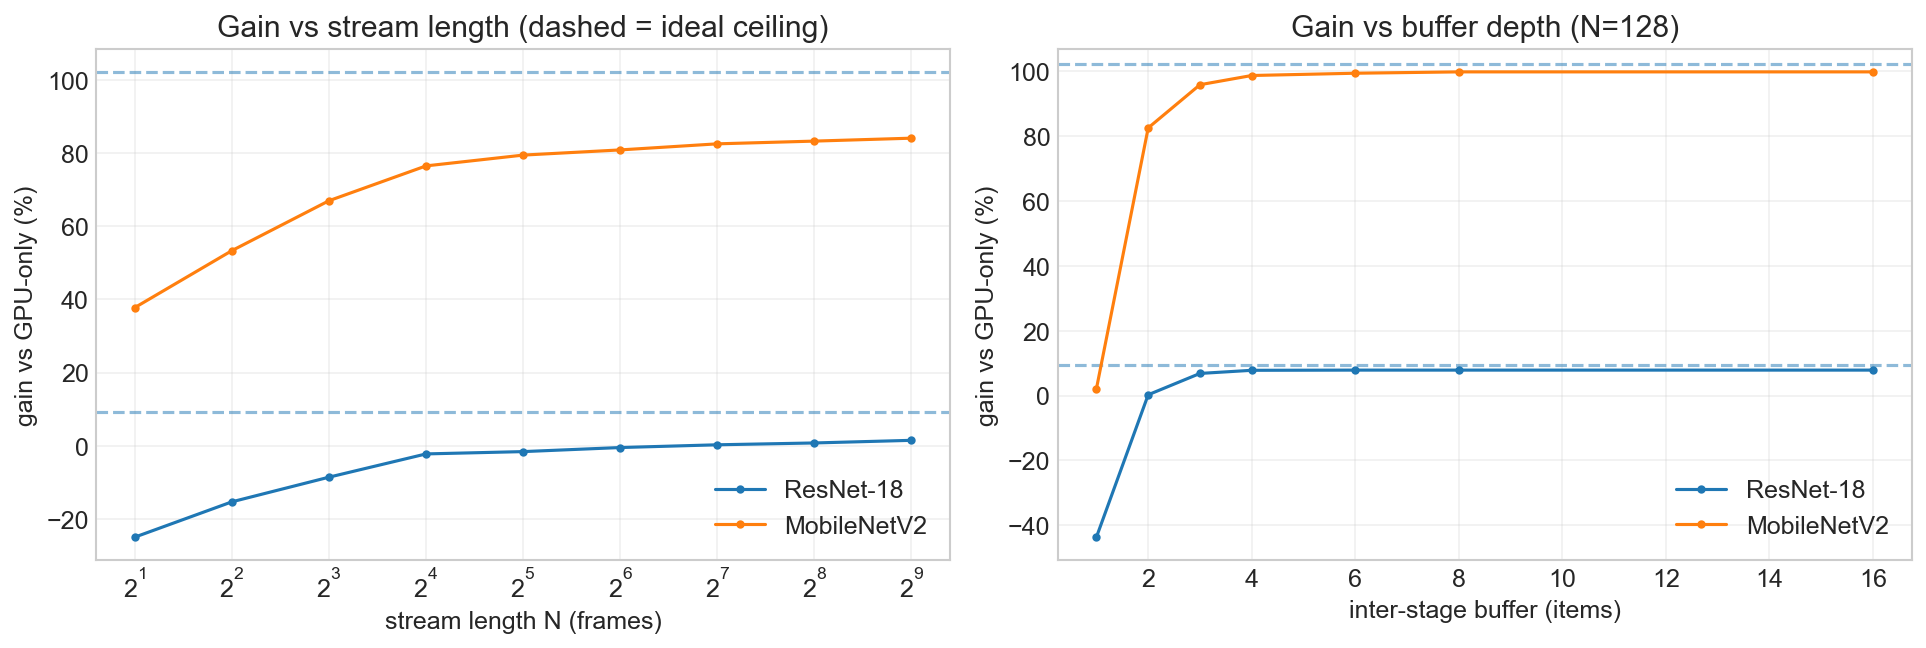
\includegraphics[width=\textwidth]{pipeline_sim.png}
\caption{Discrete-event pipeline simulation: realized gain vs stream length (left) and vs inter-stage buffer depth (right). Dashed lines mark the idealized ceilings.}\label{fig:pipesim}
\end{figure}

\subsection{Quantization Accuracy}\label{sec:accuracy}

Because the FPGA side runs INT8, an earlier split quantizes more layers. We fake-quantize (per-output-channel symmetric INT8) an increasing output-side suffix of the convolution/linear weights of pretrained torchvision models and measure agreement with the FP32 baseline (Fig.~\ref{fig:fidelity}). Fully quantized, ResNet-18 retains 100\% top-1 agreement (logit cosine 0.999) while MobileNetV2 drops to 94\% (0.997). Both architectures obtain large throughput gains, but at different fidelity cost: ResNet-18 is essentially quantization-safe (a favourable pairing, since it also gains the most throughput), whereas MobileNetV2 pays $\sim$6\% agreement for its gain---the known difficulty of quantizing depthwise-separable networks. (This is a weight-only INT8 proxy on sample inputs, indicating a fidelity trend rather than an ImageNet accuracy figure.)

\begin{figure}[t]
\centering
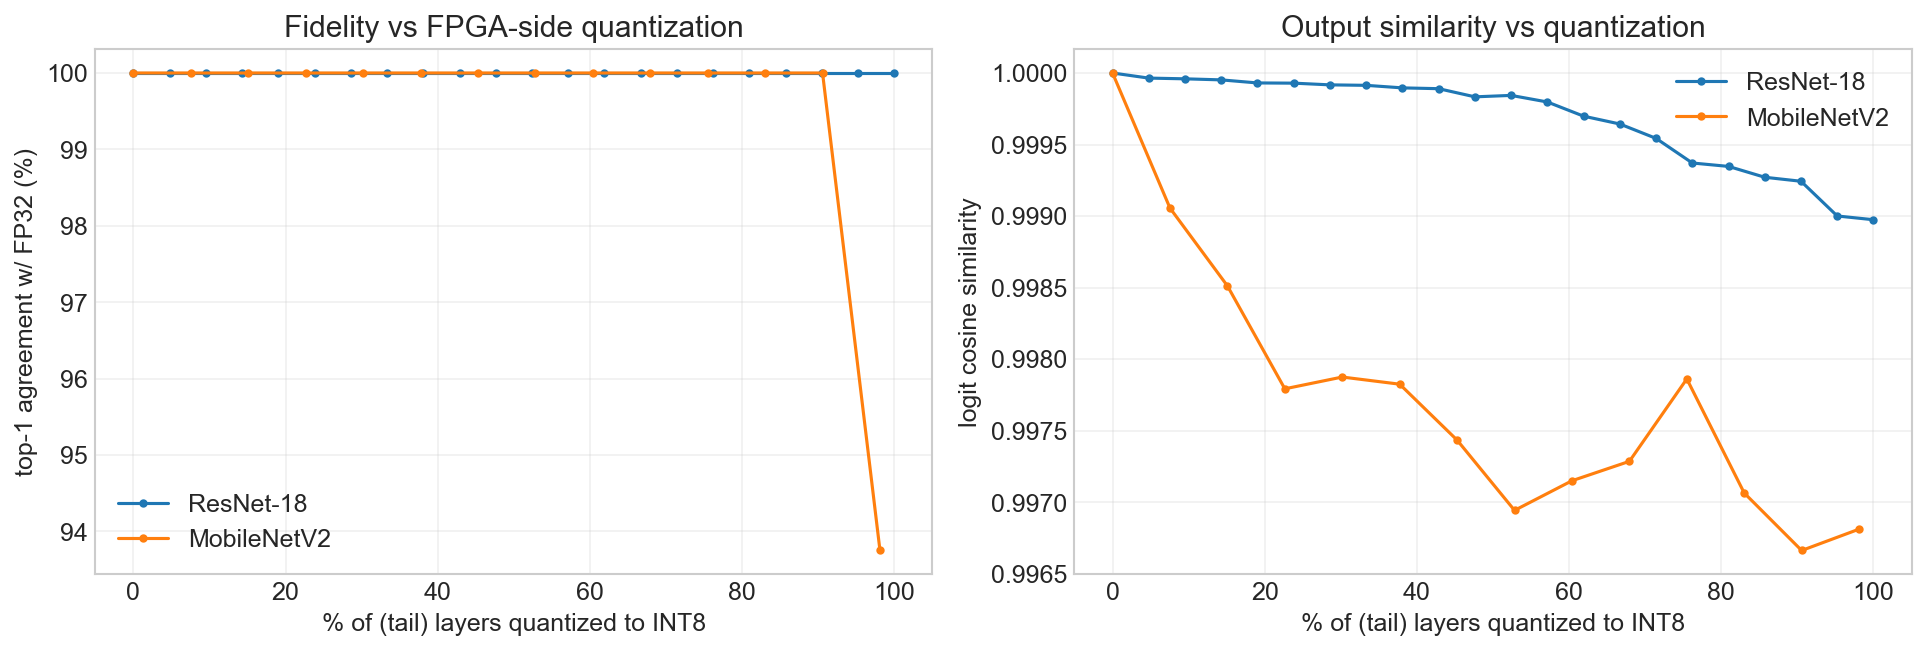
\includegraphics[width=\textwidth]{int8_fidelity.png}
\caption{INT8 fidelity vs fraction of (output-side) layers quantized: top-1 agreement with FP32 (left) and logit cosine similarity (right).}\label{fig:fidelity}
\end{figure}

\section{Discussion}\label{sec:discussion}

The multi-trial evaluation reveals that CNN inference on edge hardware is memory-bound, not compute-bound. This collapses the FPGA-to-GPU ratio from 10--37$\times$ (peak FLOPS) to 1.0--1.5$\times$ (memory-limited); analytical models relying on peak FLOPS systematically overestimate the GPU's advantage. Emulated fusion savings (47--64\% GPU, 45--77\% FPGA) far exceed the analytical 20\% for the same reason.

Calibration against published benchmarks (Section~\ref{sec:calibrated}) shows the current Zynq 7020 is too slow for positive gains in absolute terms, but break-even requires only 1.5--3$\times$, and UltraScale+ at 5--8$\times$ projects +35\% to +140\%. The hardware-grounded evaluation (Section~\ref{sec:grounded}) sharpens this picture, but it must be read on two levels. In \emph{relative} (unit-space) terms, with a properly engineered, place-and-routed convolution kernel, both architecture classes have a favourable cost structure: the tempered gains are $+132\%$ (ResNet-18) and $+81\%$ (MobileNetV2), sign-stable under uncertainty. The pivotal observation here is that an earlier naive convolution kernel---with its DSP cliff---made conv-heavy networks look marginal, and replacing it with a tiled datapath swung ResNet-18's unit-space gain by $17\times$; the relative bottleneck was the \emph{convolution datapath}, not the FPGA. In \emph{absolute} terms, however, calibration to the current Zynq~7020 is decisive: only MobileNetV2 nets a positive wall-clock gain ($+52\%$), while ResNet-18 is $-79\%$ because the device is simply too slow for its heavier compute. The two levels are consistent: the tiled conv makes conv-heavy networks \emph{structurally} suitable for offloading, but realizing that structurally-favourable split as an absolute speedup requires an FPGA at the break-even point (1.5--3$\times$ the 7020, i.e. UltraScale+ class). The honest conclusion is thus that heterogeneous execution benefits depthwise-separable networks on today's hardware and conv-heavy networks on next-generation FPGAs, with the convolution datapath---now solved---no longer the limiting factor.

The grounded evaluation also disciplines the predictor claim. The 0.20\% regret of Table~\ref{tab:predictor} is an artifact of training and testing on the same analytical formula; under leave-one-architecture-out evaluation on synthesized targets (Section~\ref{sec:b5}), regret is 0--26\%, and notably higher for the depthwise-heavy networks whose block costs are hardest to predict. This is the more trustworthy figure for a runtime scheduler. Consistently, FPGA calibration factors differ 3.2$\times$ between architectures (workload-specific implementations) while GPU varies less than 9\%---a difference the leave-one-out calibration check independently confirms.

Limitations remain. While the convolution kernel is C-simulation-verified and place-and-routed on the target part, the other operator kernels are still C-synthesis estimates rather than fully implemented, and none has been run on a physical board with a real memory hierarchy. The GPU is measured on a laptop RTX~4070 rather than the Jetson target, so only the relative per-op pattern transfers, and the fully-grounded (both-device) gain requires the cross-device calibration rather than being read directly from unit space. The pipeline simulation, while relaxing the idealized ceiling, still omits contention on shared memory interfaces, and the accuracy analysis is a weight-only proxy. End-to-end validation on a physical Zynq platform remains future work, alongside real per-layer timing on the Jetson target and extension to transformers.

\section{Conclusion}\label{sec:conclusion}

This paper presented an adaptive framework for heterogeneous GPU-FPGA CNN inference, evaluated through analytical simulation, functional emulation, and a hardware-grounded phase in which the FPGA cost model is derived from Vitis HLS synthesis for the Zynq~7020 and the GPU cost model from direct RTX~4070 measurement. The analytical model shows up to 11.8\% gain for depthwise architectures; the emulation reveals memory-bound execution, collapsing the FPGA/GPU ratio from 36.9$\times$ to 1.0$\times$; and calibration places break-even at 1.5--3$\times$ Zynq 7020 with +35\% to +140\% projected on UltraScale+. Grounding the model in synthesis with an output-stationary DSP-tiled convolution kernel (C-simulation-verified and place-and-routed on the \texttt{xc7z020}, timing met at 100~MHz), tempering the pipeline with a discrete-event simulation, and bounding the result with Monte-Carlo shows that in \emph{relative} (unit-space) terms both depthwise-separable ($+81\%$) and conv-heavy ($+132\%$) networks have a favourable, sign-stable structure---a naive convolution kernel had hidden this for conv-heavy networks, and the $17\times$ swing on replacing it identifies the convolution datapath, not the device, as the bottleneck. Calibrating to \emph{absolute} time on the current Zynq~7020 is stricter: only MobileNetV2 is net-positive ($+52\%$), while ResNet-18 ($-79\%$) needs an UltraScale+-class FPGA (the break-even point) to convert its favourable structure into a wall-clock win. The same grounding corrects the predictor result to a realistic 0--26\% scheduling regret. The framework adapts automatically from conservative tail splits to aggressive partitioning as the balance between the two devices shifts.

\appendix

\newpage
\section{Supplementary Figures}\label{sec:appendix}

\subsection{Trial 1: Analytical Simulation}

\begin{figure}[!htpb]
\centering
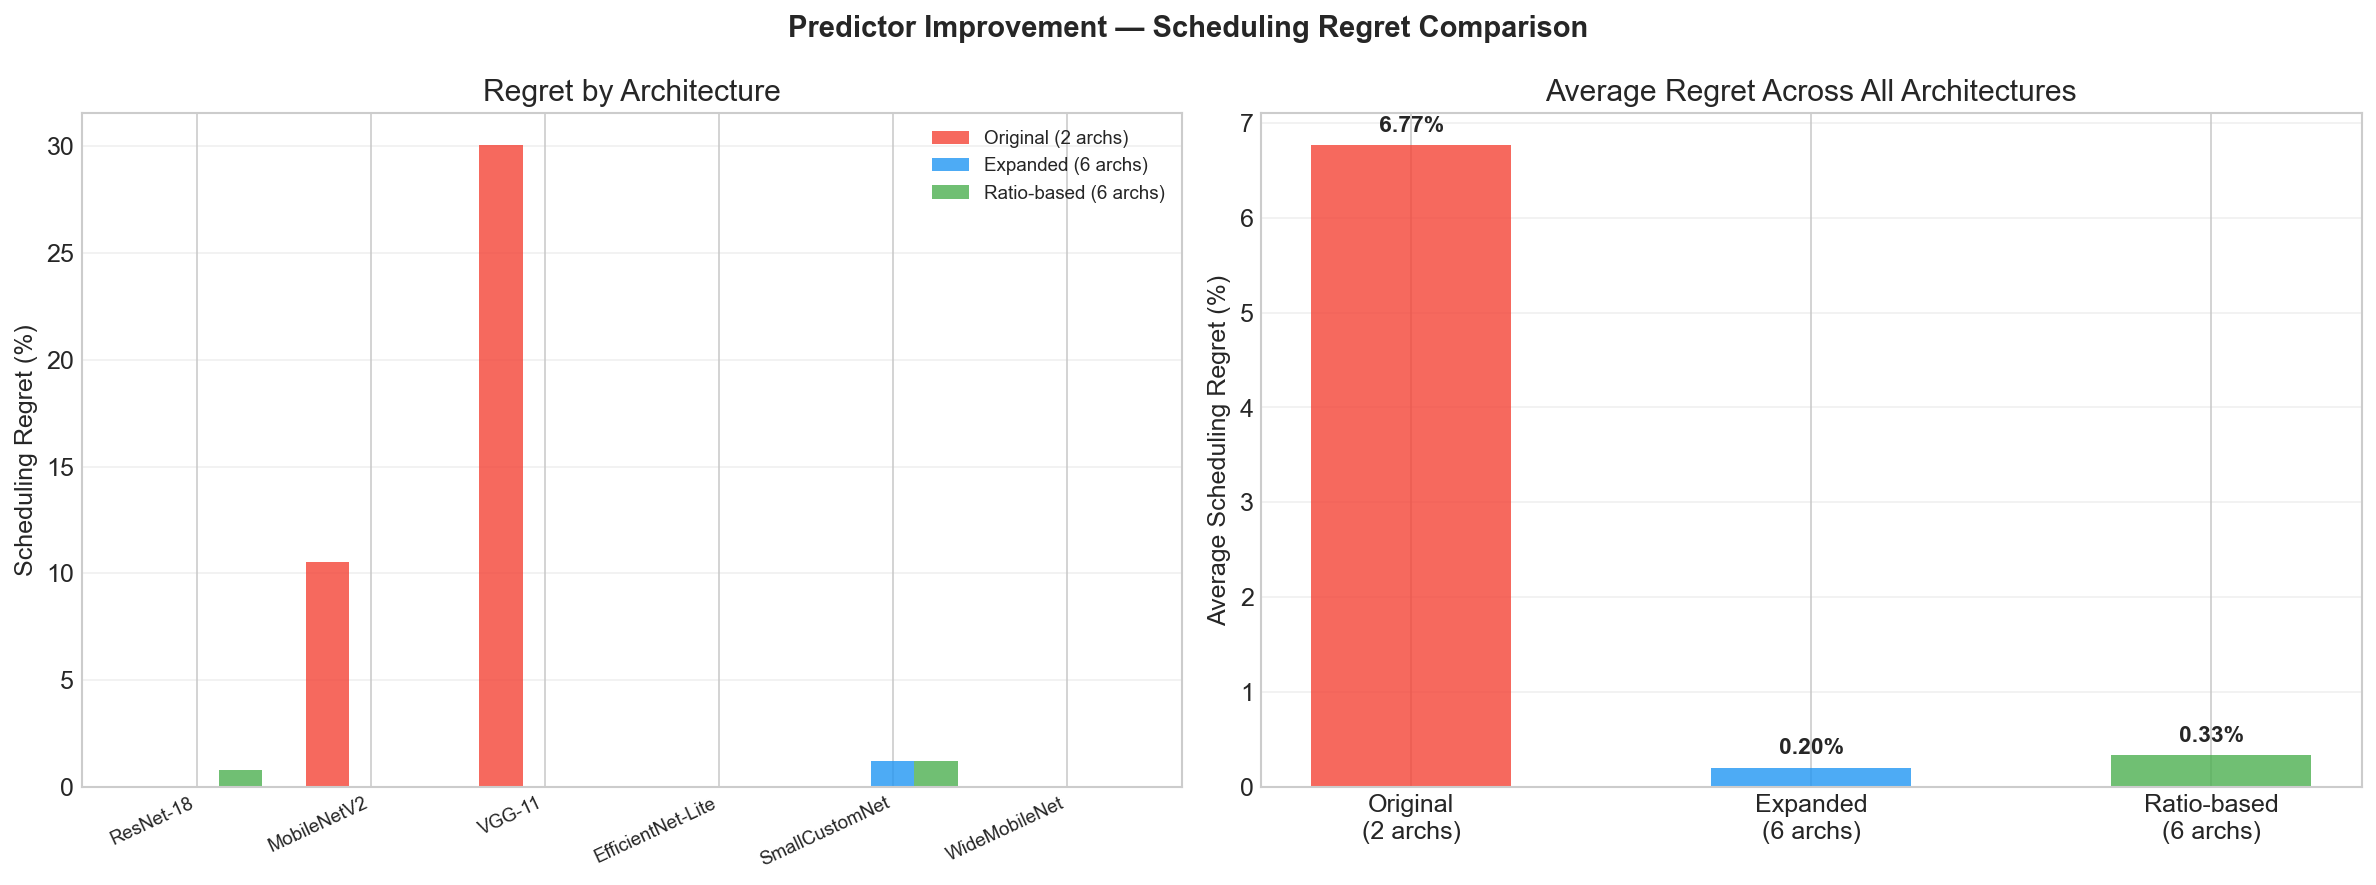
\includegraphics[width=\textwidth, height=0.35\textheight, keepaspectratio]{predictor_improvement_comparison.png}
\caption{Predictor scheduling regret: original (2 architectures) vs expanded (6 architectures) training, under the in-model protocol (cf. Section~\ref{sec:b5} for the grounded, cross-validated evaluation).}\label{fig:t1_predictor}
\end{figure}

\begin{figure}[!htpb]
\centering
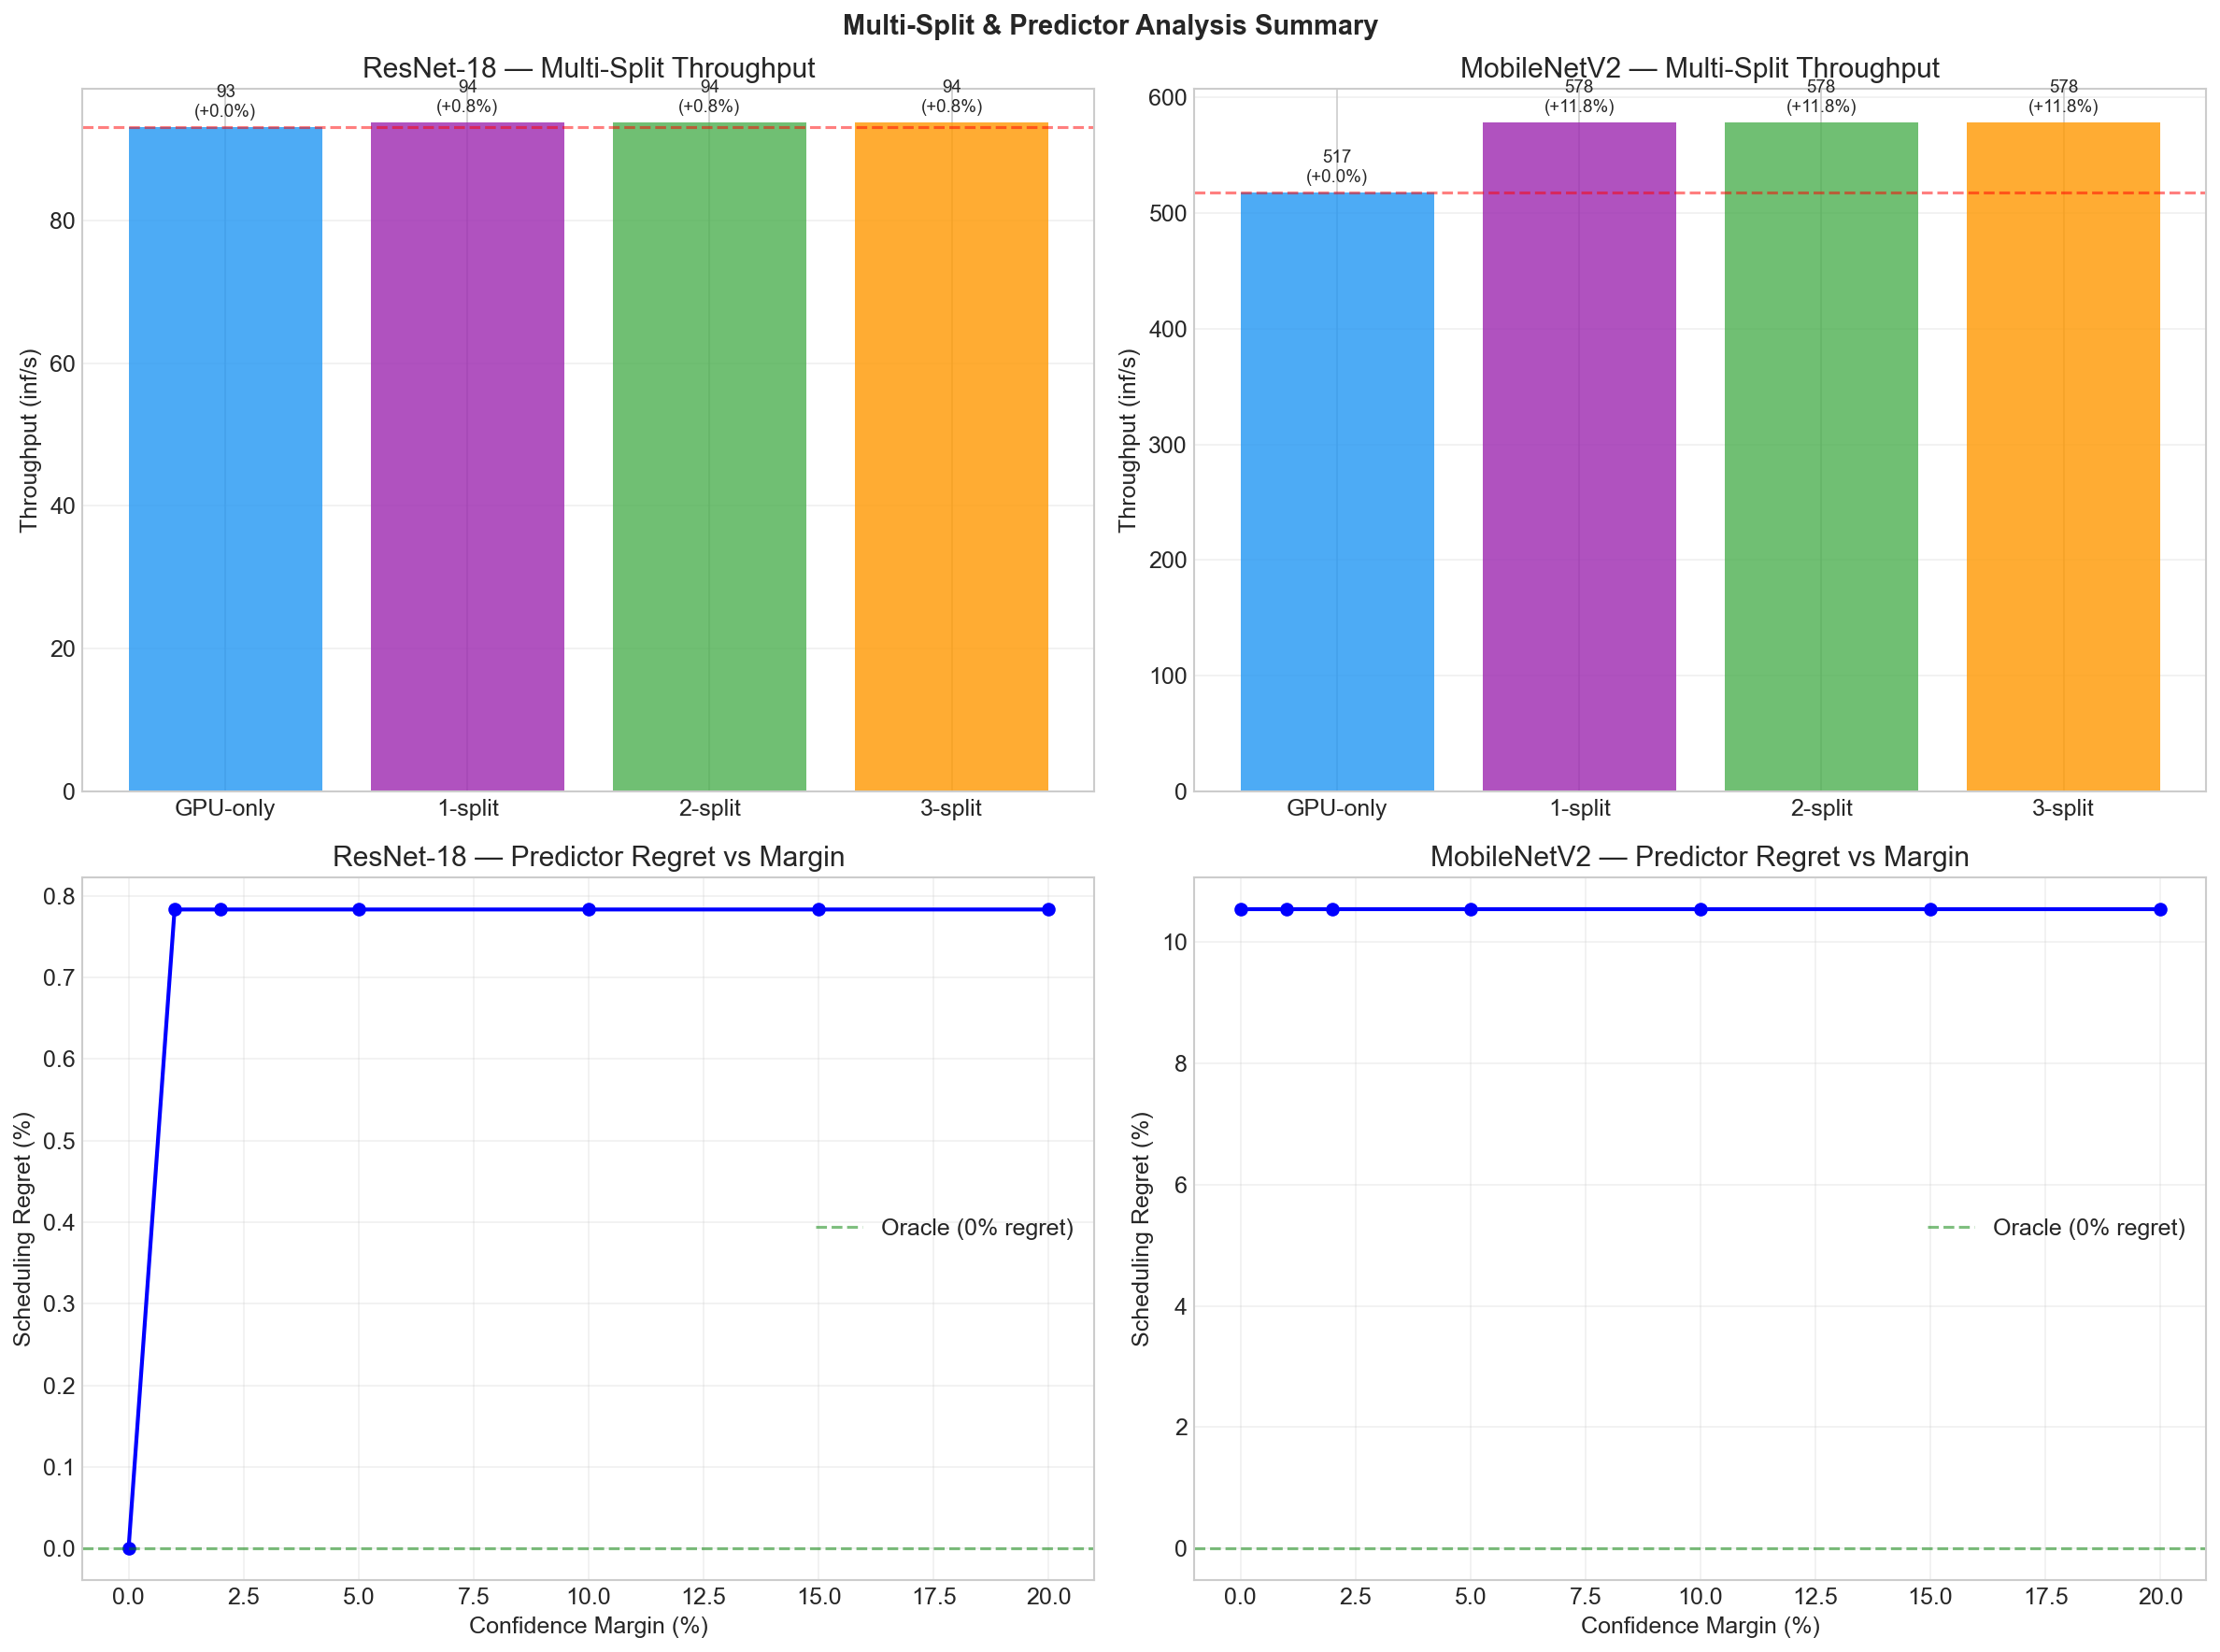
\includegraphics[width=\textwidth, height=0.35\textheight, keepaspectratio]{multi_split_and_predictor_summary.png}
\caption{Multi-split throughput comparison (top) and predictor regret vs confidence margin (bottom). Single-split is sufficient at current FPGA performance levels.}\label{fig:t1_multisplit}
\end{figure}

\clearpage
\subsection{Trial 2: Functional Emulation}

\begin{figure}[!htpb]
\centering
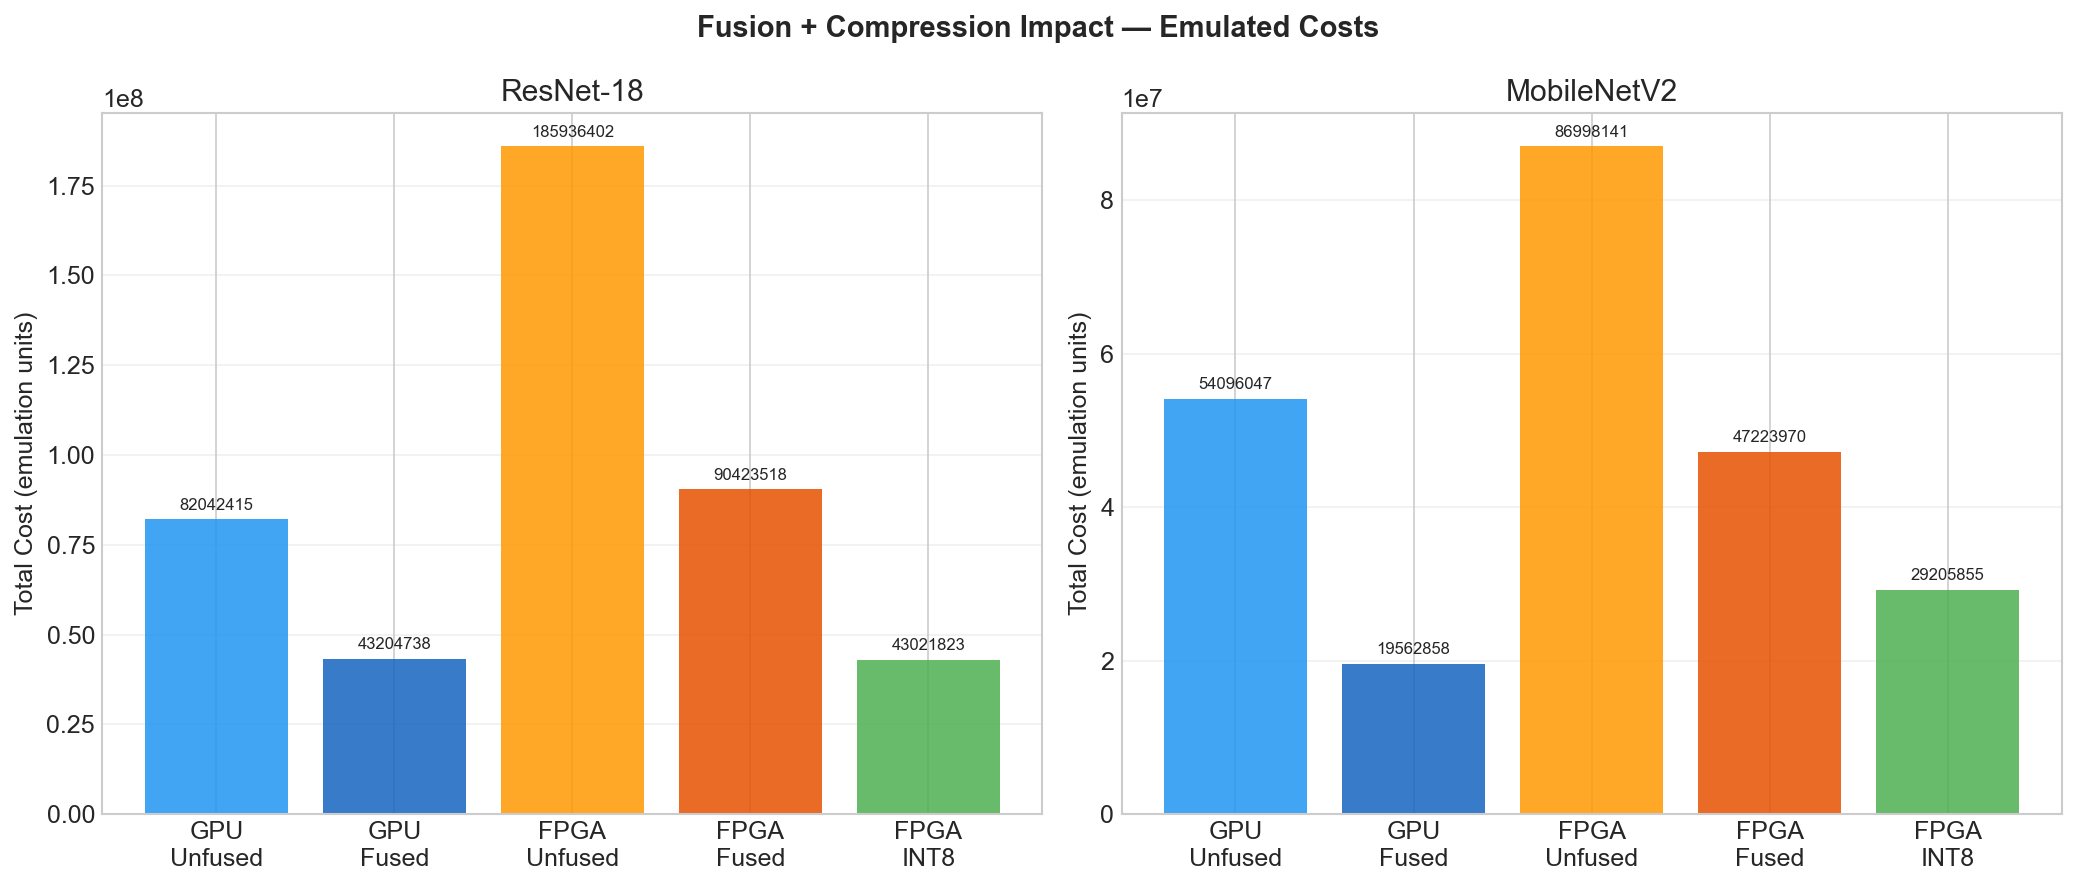
\includegraphics[width=\textwidth, height=0.20\textheight, keepaspectratio]{fusion_compression_impact.png}
\caption{Fusion and INT8 compression impact on emulated cost.}\label{fig:t2_fusion}
\end{figure}

\begin{figure}[!htpb]
\centering
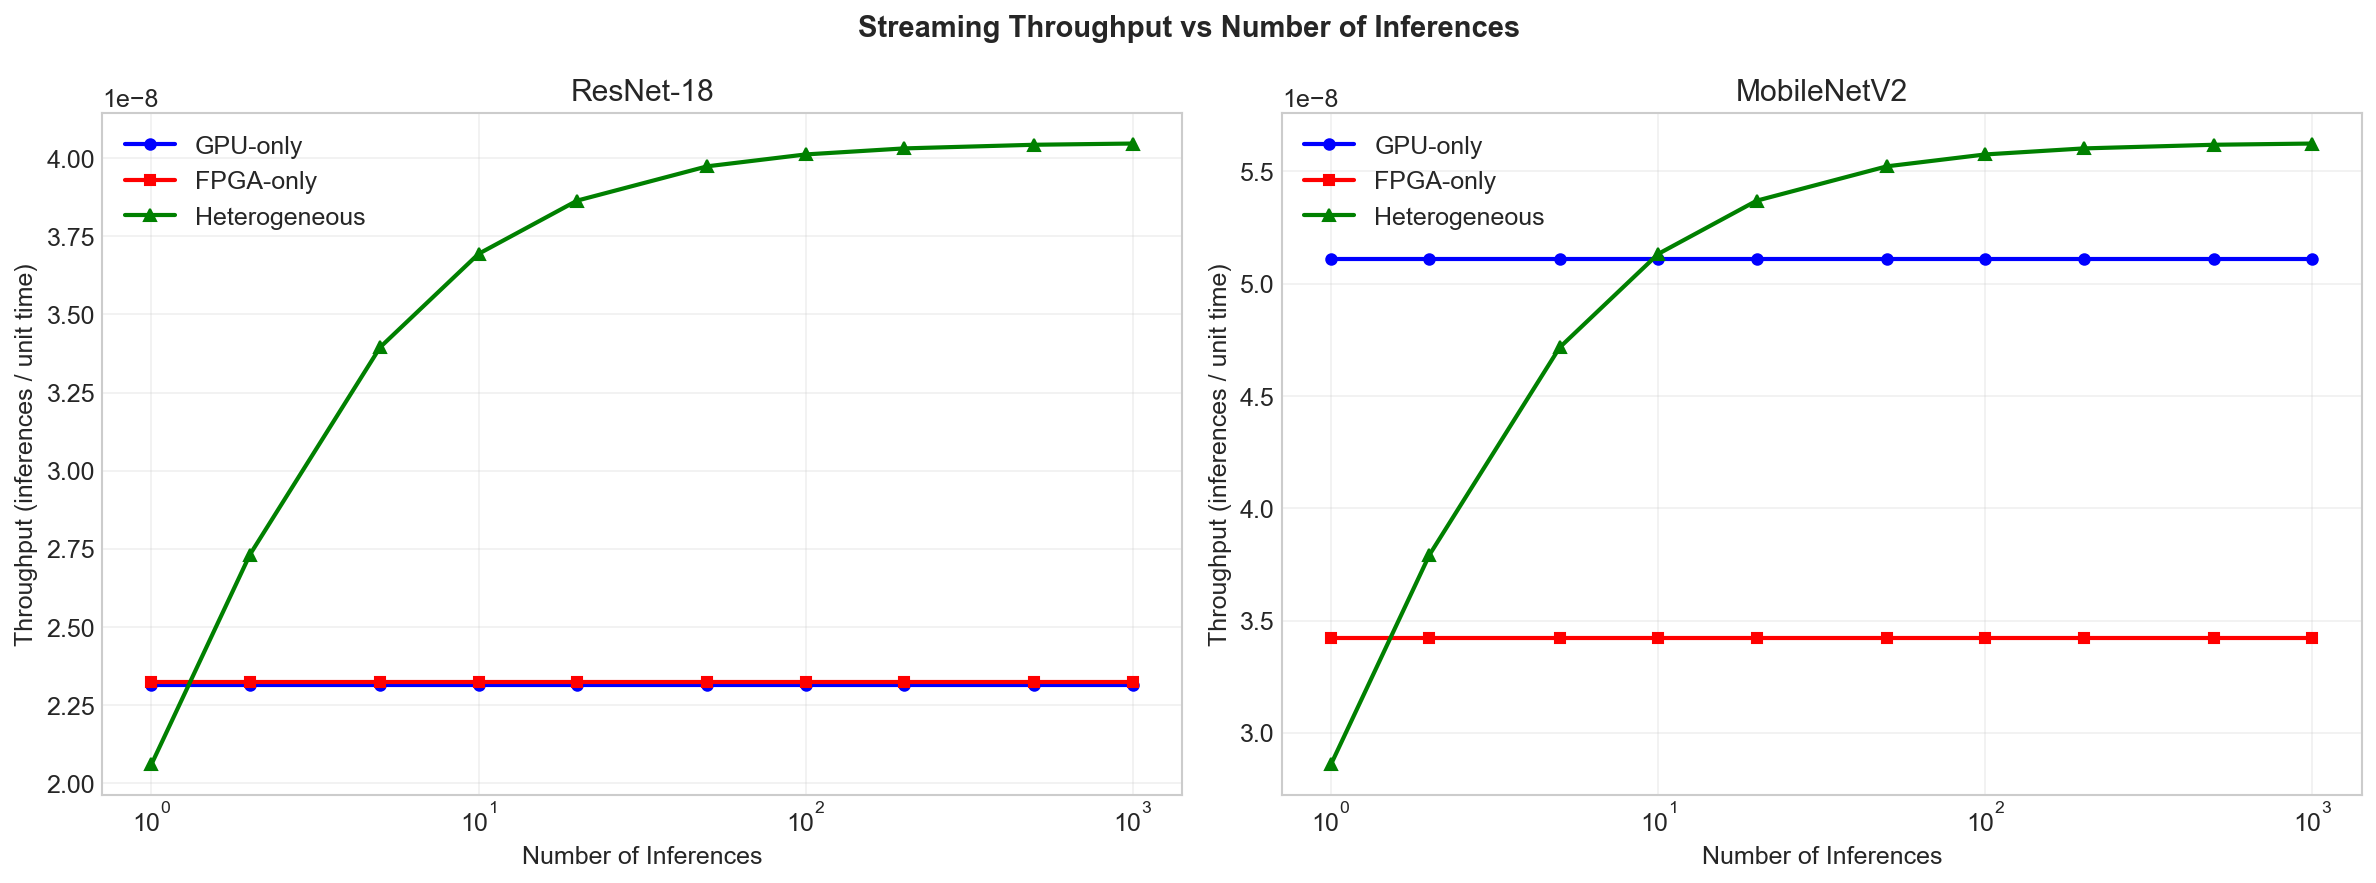
\includegraphics[width=0.85\textwidth, height=0.20\textheight, keepaspectratio]{streaming_throughput_vs_length.png}
\caption{Streaming throughput vs number of inferences (emulation).}\label{fig:t2_streaming}
\end{figure}

\begin{figure}[!htpb]
\centering
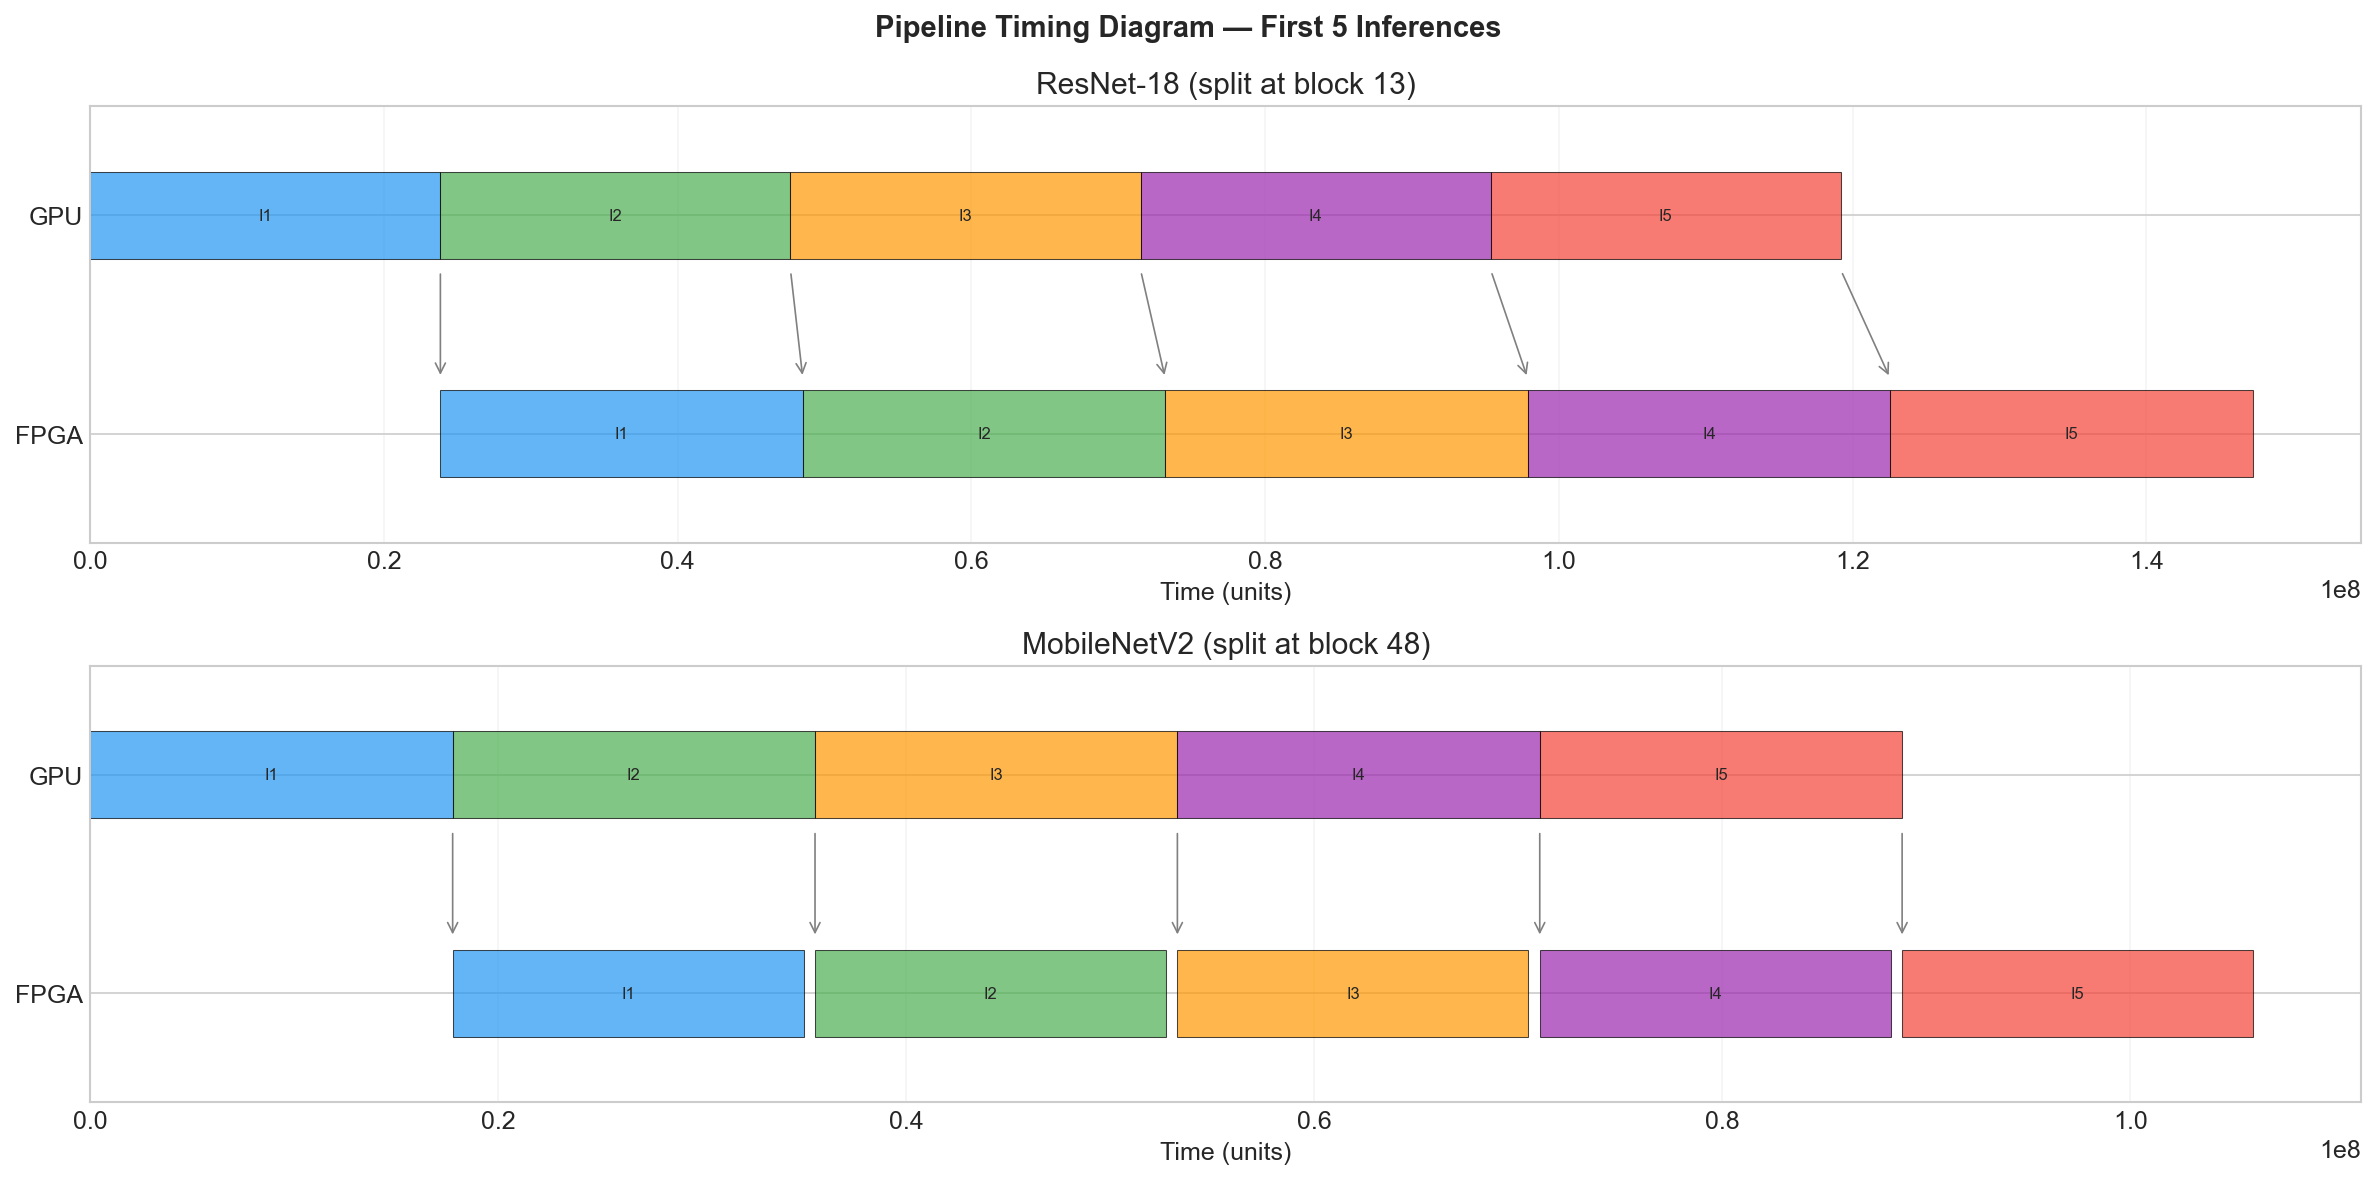
\includegraphics[width=0.85\textwidth, height=0.20\textheight, keepaspectratio]{pipeline_timing_diagram.png}
\caption{Emulated pipeline timing showing overlapping GPU and FPGA execution for the first 5 inferences. Each color represents one input frame.}\label{fig:t2_pipeline}
\end{figure}

\clearpage
\subsection{Calibrated Emulation Results}

\begin{figure}[!htpb]
\centering
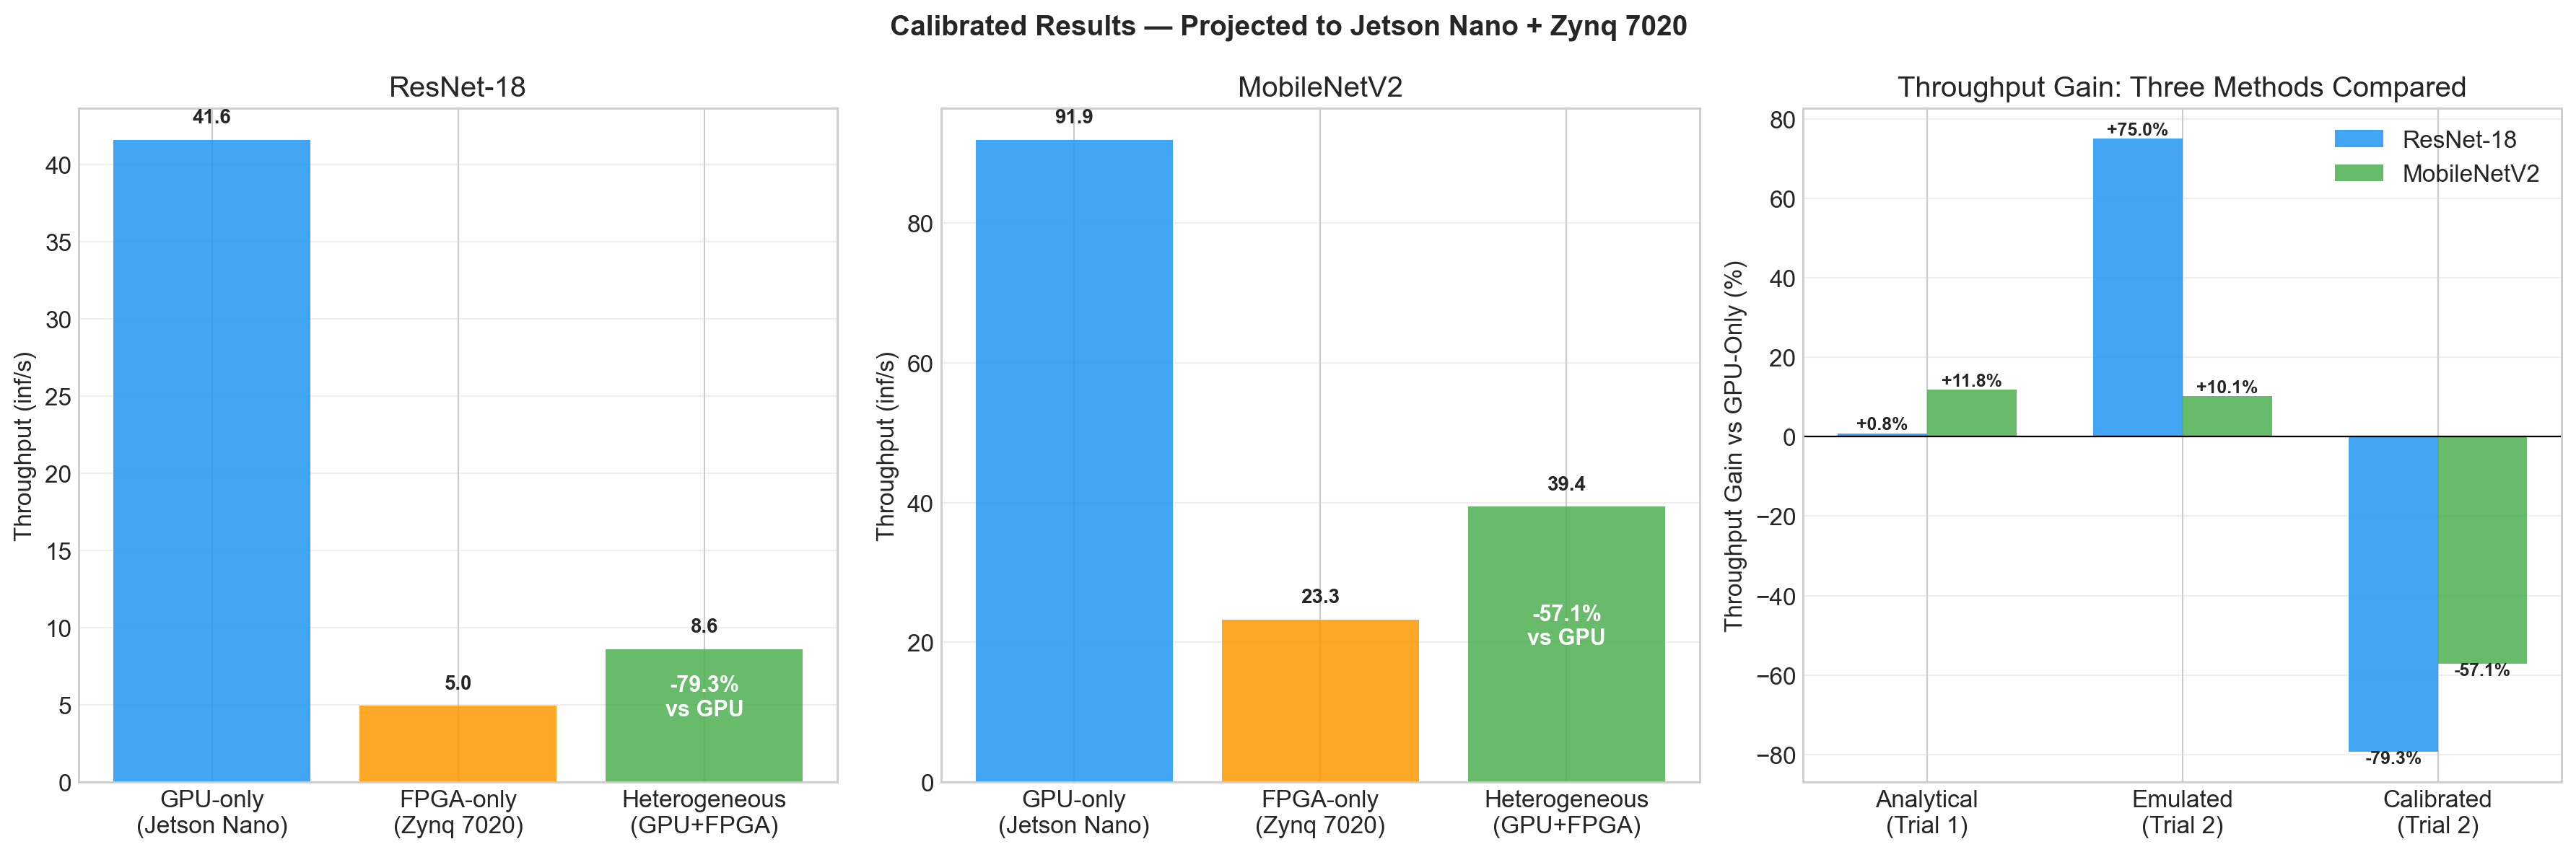
\includegraphics[width=\textwidth, height=0.35\textheight, keepaspectratio]{calibrated_results_corrected.png}
\caption{Trial 2 calibrated results: (a,b) projected throughput on Jetson Nano + Zynq 7020 target hardware, (c) throughput gain comparison across analytical, emulated, and calibrated modeling levels.}\label{fig:t2_calibrated}
\end{figure}

\begin{figure}[!htpb]
\centering
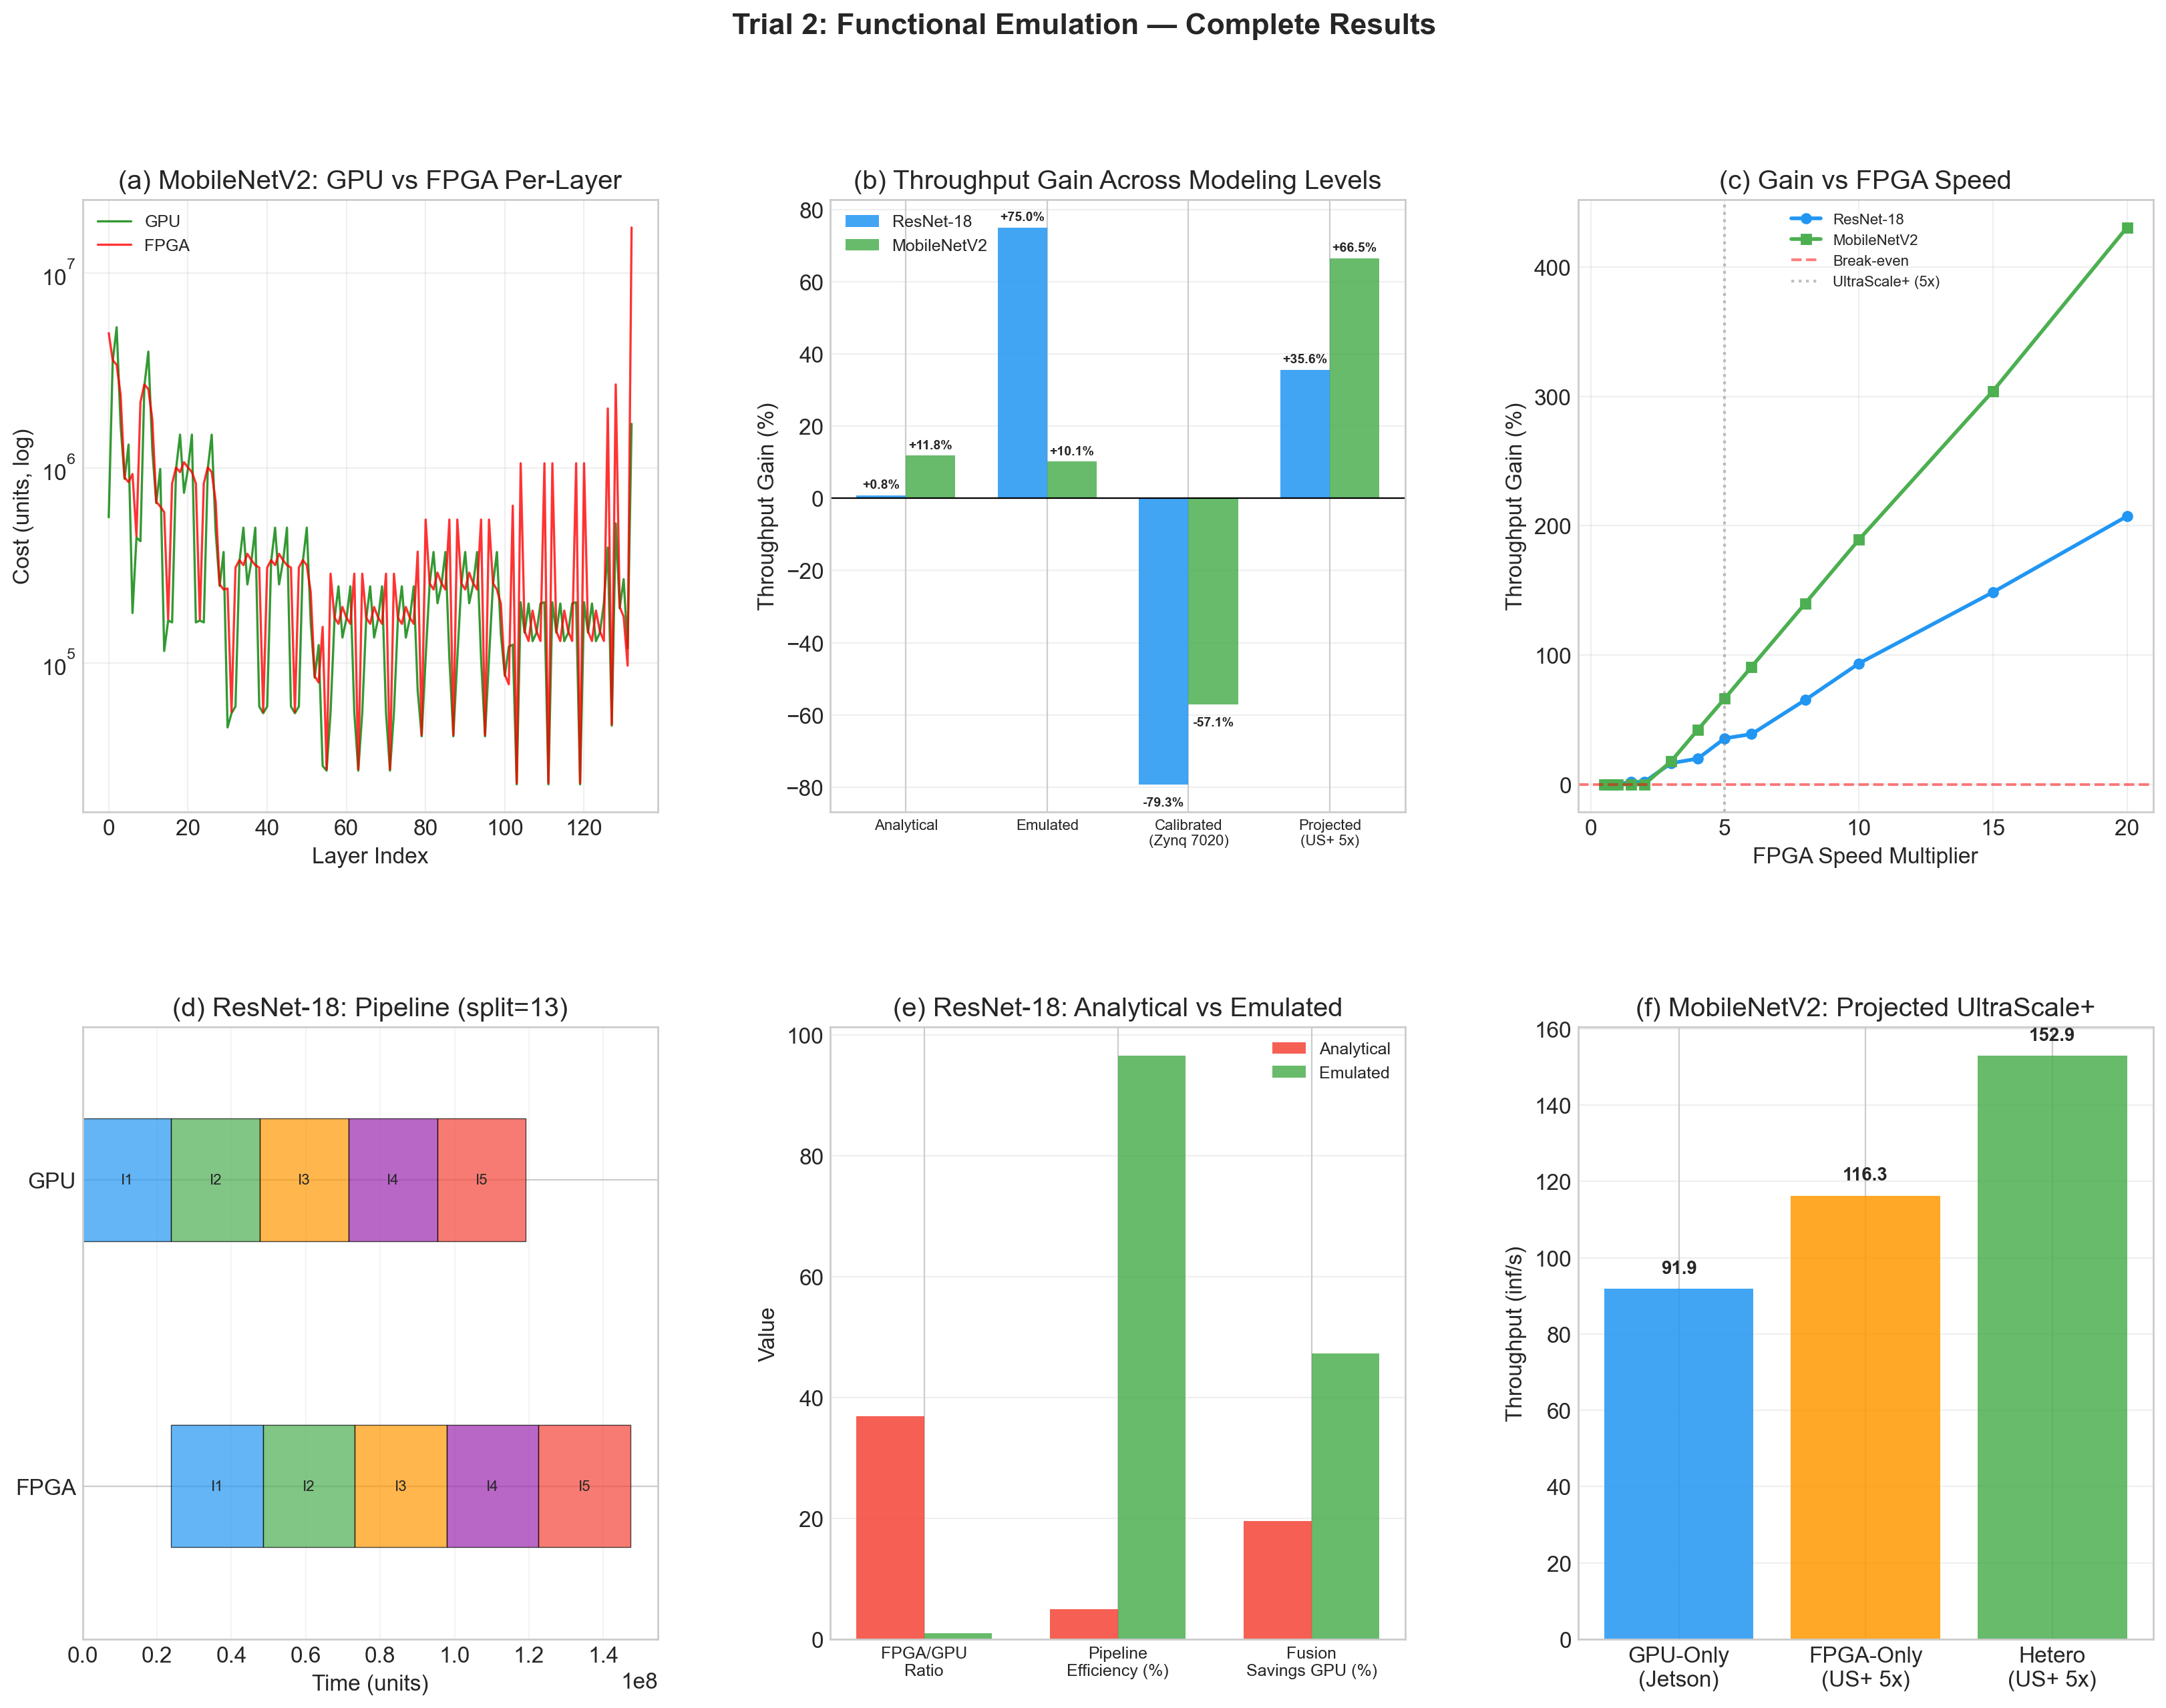
\includegraphics[width=\textwidth, height=0.35\textheight, keepaspectratio]{trial2_final_summary.png}
\caption{Trial 2 complete summary: (a) per-layer GPU vs FPGA costs, (b) four-level throughput gain comparison, (c) gain vs FPGA speed, (d) pipeline timing, (e) analytical vs emulated metrics, (f) UltraScale+ projected throughput.}\label{fig:t2_final}
\end{figure}

\begin{thebibliography}{99}

\bibitem{he2016} He, K., Zhang, X., Ren, S., Sun, J.: Deep residual learning for image recognition. In: IEEE Conf. on Computer Vision and Pattern Recognition (CVPR), pp. 770--778 (2016)

\bibitem{sandler2018} Sandler, M., Howard, A., Zhu, M., Zhmoginov, A., Chen, L.C.: MobileNetV2: Inverted residuals and linear bottlenecks. In: IEEE Conf. on Computer Vision and Pattern Recognition (CVPR), pp. 4510--4520 (2018)

\bibitem{howard2017} Howard, A.G., Zhu, M., Chen, B., Kalenichenko, D., Wang, W., Weyand, T., Andreetto, M., Adam, H.: MobileNets: Efficient convolutional neural networks for mobile vision applications. arXiv:1704.04861 (2017)

\bibitem{roofline2009} Williams, S., Waterman, A., Patterson, D.: Roofline: An insightful visual performance model for multicore architectures. Communications of the ACM 52(4), 65--76 (2009)

\bibitem{ioffe2015} Ioffe, S., Szegedy, C.: Batch normalization: Accelerating deep network training by reducing internal covariate shift. In: Int. Conf. on Machine Learning (ICML), pp. 448--456 (2015)

\bibitem{jacob2018} Jacob, B., Kligys, S., Chen, B., Zhu, M., Tang, M., Howard, A., Adam, H., Kalenichenko, D.: Quantization and training of neural networks for efficient integer-arithmetic-only inference. In: IEEE Conf. on Computer Vision and Pattern Recognition (CVPR), pp. 2704--2713 (2018)

\bibitem{krishnamoorthi2018} Krishnamoorthi, R.: Quantizing deep convolutional networks for efficient inference: A whitepaper. arXiv:1806.08342 (2018)

\bibitem{zhang2015} Zhang, C., Li, P., Sun, G., Guan, Y., Xiao, B., Cong, J.: Optimizing FPGA-based accelerator design for deep convolutional neural networks. In: ACM/SIGDA Int. Symp. on Field-Programmable Gate Arrays (FPGA), pp. 161--170 (2015)

\bibitem{qiu2016} Qiu, J., Wang, J., Yao, S., Guo, K., Li, B., Zhou, E., Yu, J., Tang, T., Xu, N., Song, S., Wang, Y., Yang, H.: Going deeper with embedded FPGA platform for convolutional neural network. In: ACM/SIGDA Int. Symp. on Field-Programmable Gate Arrays (FPGA), pp. 26--35 (2016)

\bibitem{finn2017} Umuroglu, Y., Fraser, N.J., Gambardella, G., Blott, M., Leong, P., Jahre, M., Vissers, K.: FINN: A framework for fast, scalable binarized neural network inference. In: ACM/SIGDA Int. Symp. on Field-Programmable Gate Arrays (FPGA), pp. 65--74 (2017)

\bibitem{hls4ml2018} Duarte, J., et al.: Fast inference of deep neural networks in FPGAs for particle physics. Journal of Instrumentation 13(07), P07027 (2018)

\bibitem{eyeriss2017} Chen, Y.H., Krishna, T., Emer, J.S., Sze, V.: Eyeriss: An energy-efficient reconfigurable accelerator for deep convolutional neural networks. IEEE Journal of Solid-State Circuits 52(1), 127--138 (2017)

\bibitem{guo2019} Guo, K., Zeng, S., Yu, J., Wang, Y., Yang, H.: A survey of FPGA-based neural network inference accelerators. ACM Transactions on Reconfigurable Technology and Systems 12(1), 1--26 (2019)

\bibitem{neurosurgeon2017} Kang, Y., Hauswald, J., Gao, C., Rovinski, A., Mudge, T., Mars, J., Tang, L.: Neurosurgeon: Collaborative intelligence between the cloud and mobile edge. In: ACM Int. Conf. on Architectural Support for Programming Languages and Operating Systems (ASPLOS), pp. 615--629 (2017)

\bibitem{matsubara2022} Matsubara, Y., Levorato, M., Restuccia, F.: Split computing and early exiting for deep learning applications: Survey and research challenges. ACM Computing Surveys 55(5), 1--30 (2022)

\bibitem{tvm2018} Chen, T., Moreau, T., Jiang, Z., Zheng, L., Yan, E., Cowan, M., Shen, H., Wang, L., Hu, Y., Ceze, L., Guestrin, C., Krishnamurthy, A.: TVM: An automated end-to-end optimizing compiler for deep learning. In: USENIX Symp. on Operating Systems Design and Implementation (OSDI), pp. 578--594 (2018)

\bibitem{vitishls} AMD/Xilinx: Vitis High-Level Synthesis User Guide (UG1399). Advanced Micro Devices, Inc. (2023)

\bibitem{deepedgebench2021} Baller, S.P., Jindal, A., Chadha, A., Chinnusamy, M.: DeepEdgeBench: Benchmarking deep neural networks on edge devices. In: IEEE Int. Conf. on Cloud Engineering (IC2E), pp. 20--30 (2021)

\bibitem{tensorrt} NVIDIA Corporation: NVIDIA TensorRT: Programmable inference accelerator. \url{https://developer.nvidia.com/tensorrt} (accessed 2026)

\end{thebibliography}

\end{document}
